% This template originates from the Cambridge University thesis 
% which is created by Prof Harish Bhanderi.  
% This is template follows the GNU license for Education and training
% purposes. (http://www-h.eng.cam.ac.uk/help/tpl/textprocessing/ThesisStyle/) 
% 
%
% I modified for uses in University of Information Technology 
% Vietnam National University. 

\documentclass[oneside,12pt]{Classes/uitBA}

\usepackage{cite}
\usepackage{graphicx}
\usepackage{caption}
\usepackage{booktabs} % For \toprule, \midrule and \bottomrule
\usepackage{pgfplotstable} % Generates table from .csv

\newcommand{\head}[1]{\textnormal{\textbf{#1}}}



 \ifpdf
     \pdfinfo { /Title  (Thesis title)
                /Creator (TeX)
                /Producer (pdfTeX)
                /Author (Nguyen Van X, Nguyen Van Y)
                /CreationDate (D:20121211000000)  %format D:YYYYMMDDhhmmss
                /ModDate (D:20030815213532)
                /Subject (Thesis title)
                /Keywords (PhD, Thesis)}
     \pdfcatalog { /PageMode (/UseOutlines)
                   /OpenAction (fitbh)  }
 \fi
     
  \university{{ĐẠI HỌC QUỐC GIA THÀNH PHỐ HỒ CHÍ MINH\\
               ĐẠI HỌC CÔNG NGHỆ THÔNG TIN}}
  \collegeordept{{KHOA KHOA HỌC MÁY TÍNH}}  
  \degree{CỬ NHÂN CÔNG NGHỆ THÔNG TIN}   
  \title{KHÓA LUẬN TỐT NGHIỆP\\
  PHÂN LỚP VẬT LIỆU BỀ SỬ DỤNG MẠNG HỌC SÂU} 
  \crest{
\includegraphics[scale=.20]{UITLogo}} 
  \supervisor{{TS. MAI TIẾN DŨNG
  				\\ TS. LÊ ĐÌNH DUY}}
  \author{{TRƯƠNG PHÚC ANH - 14520040}}   
  \degreedate{6, 2018} 
\hbadness=10000
\hfuzz=50pt
\usepackage{StyleFiles/watermark}
\onehalfspacing

\begin{document}
\maketitle
\setcounter{secnumdepth}{3}
\setcounter{tocdepth}{3}

\frontmatter % book mode only
\pagenumbering{roman}
\begin{dedication}  

Xin dành tặng quyển luận văn này cho ... 

\end{dedication}

 
\begin{acknowledgements}      

Sau quá trình học tập và rèn luyện tại trường Đại học Công Nghệ Thông Tin, Khoa Khoa Học Máy Tính và 4 tháng thực hiện đề tài nghiên cứu này, em xin tỏ lòng cảm ơn chân thành đến các thầy, cô giảng viên, cán bộ các phòng, ban chức năng tại trường đã giúp đỡ em hoàn thành luận văn tốt nghiệp này.

Đặc biệt, em chân thành cảm ơn thầy Mai Tiến Dũng và Lê Đình Duy đã chỉ bảo, hướng dẫn và giúp đỡ em rất nhiều trong suốt quá trình thực hiện đề tài. Một lần nữa em chân thành cảm ơn và chúc các thầy dồi dào sức khoẻ.

Em cũng xin cảm ơn tất cả các bạn bè, anh chị đang học tập và làm việc tại trường, đặc biệt là MMLab đã nhiệt tình giúp đỡ em trong suốt thời gian qua.

Tuy nhiên vì kiến thức chuyên môn còn hạn chế và bản thân còn thiếu nhiều kinh nghiệm thực tiễn nên nội dung của báo cáo không tránh khỏi những thiếu xót, em rất mong nhận sự góp ý, chỉ bảo thêm của quý thầy cô để báo cáo này được hoàn thiện hơn.

\end{acknowledgements}

\paragraph*{}
In real world, materials have rich surface texture, geometry, lighting conditions, and clutter, which combine to make the problem more challanging.

\tableofcontents
\listoffigures
 \printnomenclature  
 \addcontentsline{toc}{chapter}{Nomenclature}

\mainmatter  
% \pagebreak[4]
% \hspace*{1cm}
% \pagebreak[4]
% \hspace*{1cm}
% \pagebreak[4]

\chapter{Mở đầu}
\ifpdf
    \graphicspath{{Chapter1/Chapter1Figs/PNG/}{Chapter1/Chapter1Figs/PDF/}{Chapter1/Chapter1Figs/}}
\else
    \graphicspath{{Chapter1/Chapter1Figs/EPS/}{Chapter1/Chapter1Figs/}}
\fi

\section{Giới thiệu bài toán}
Mục tiêu chính của bài toán phân lớp vật liệu là cung cấp thông tin vật liệu càng chi tiết càng tốt của một đối tượng hoặc một bề mặt trong ảnh. Hiểu một cách đơn giản, cho trước một ảnh I, máy tính cần trả lời câu hỏi "Đối tượng (hay bề mặt này) được làm từ vật liệu gì?" (chẳng hạn như gỗ, giấy, đá, kim loại, ...) (Hình \ref{fig:problem}). Ở một cấp độ cao hơn của bài toán, máy tính cần cho biết chính xác loại vật liệu của từng pixel trên ảnh (Hình \ref{fig:seg}). Trong luận văn này, nhóm giải quyết câu hỏi thứ nhất.

\begin{figure}[h!]
	\centering
	\captionsetup{width=0.9\textwidth}
	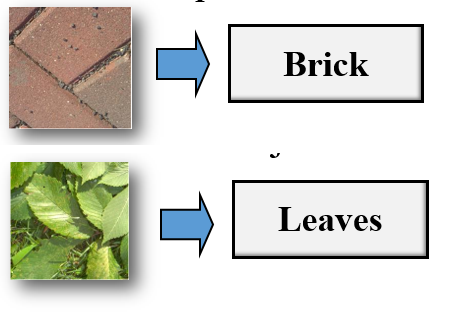
\includegraphics[width=0.5\textwidth]{problem.png}
	\caption{Phân lớp vật liệu cho biết bề mặt trong ảnh thuộc vật liệu nào}
    \label{fig:problem}
\end{figure}

\begin{figure}[h!]
	\centering
	\captionsetup{width=0.9\textwidth}
	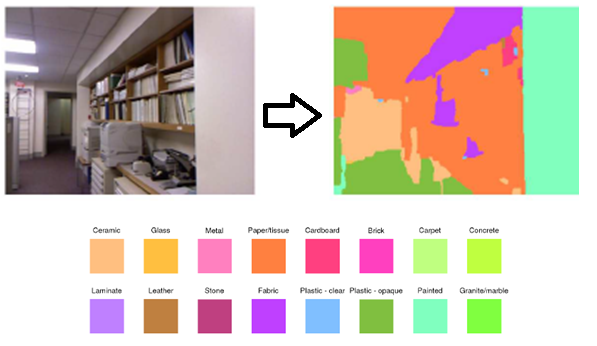
\includegraphics[width=0.8\textwidth]{segmentation.png}
	\caption{Phân lớp vật liệu cho biết chính xác vật liệu của từng pixel trong ảnh}
    \label{fig:seg}
\end{figure}

\pagebreak

\section{Tại sao cần phân lớp vật liệu?}
\paragraph*{}
Vật liệu của một bề mặt hay đối tượng nào đó là một thông tin rất giá trị để máy tính của thể hiểu được các thuộc tính của nó và từ đó có thể đưa ra các quyết định liên quan cũng như tương tác với chúng. Hình \ref{fig:bottles} và \ref{fig:car} là hai ví dụ đơn giản cho thấy máy tính có thể làm được rất nhiều việc khi có thể biết được thông tin về vật liệu. Trong hình \ref{fig:bottles}, với thông tin về vật liệu của các chai nước này này, đơn giản nhất máy tính có thể sắp xếp chúng theo cân nặng, ngoài ra còn có thể quyết định chai nào có thể được dùng để đựng nước nóng chai nào không thể hay thậm chí chai nào có thể sử dụng để gây sát thương cho người khác (chai thủy tinh

\begin{figure}[h!]
	\centering
	\captionsetup{width=0.9\textwidth}
	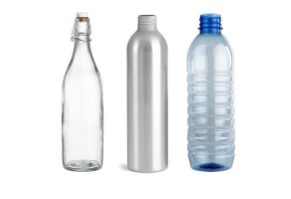
\includegraphics[width=0.8\textwidth]{bottles.png}
	\caption{Ba chai đựng nước với hình dáng tương tự nhau được làm từ những vật liệu khác nhau - quyết định những tính chất vật lý khác nhau}
    \label{fig:bottles}
\end{figure}

\begin{figure}[h!]
	\centering
	\captionsetup{width=0.9\textwidth}
	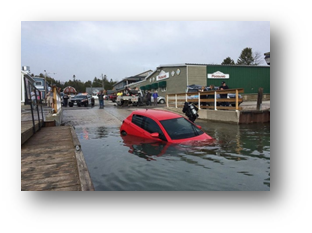
\includegraphics[width=0.8\textwidth]{car.png}
	\caption{Xe tự lái: "Xin lỗi, tôi không biết đó là nước :("}
    \label{fig:car}
\end{figure}

\paragraph*{}
Ngoài ra, vật liệu còn là một chìa khóa quan trọng để cải tiến bài toán "Scene understanding" trong Thị Giác Máy Tính \cite{corbettreal} và còn được ứng dụng trong nhiều lĩnh vực khác nhau trong đời sống như các hệ thống xe tự lái (Advanced Driver-Assistance Systems) \cite{r1}, Robotic Manipulation \cite{spong2006robot} hay Robotic Navigation \cite{kim2013robot}. 

\section{Các thách thức của bài toán}
Nhiều thách thức khác nhau kết hợp làm bài toán phân lớp vật liệu rất khó giải quyết triệt để. Sự đa dạng về hình dáng, kích thước và texture là một trong số đó, có rất nhiều đối tượng có hình dáng khác nhau nhưng lại cùng loại vật liệu, ngược lại có những đối tượng trông có vẽ rất giống nhau nhưng lại làm từ những vật liệu khác nhau. Ngoài ra, điều kiện chiếu sáng khác nhau cũng khiến việc phân biệt giữa các vật liệu trở nên rất khó khăn (đặc biết đối với việc chỉ dùng một ảnh màu để phân biệt). Bên cạnh đó, sự chồng lắp giữa các đối tượng với nhau, giữa đối tượng với background cũng là một thách thức không nhỏ. Hình \ref{ex1} và \ref{ex2} là hai ví dụ cho thấy bài toán này thật sự rất thách thức.

\begin{figure}[h!]
	\centering
	\captionsetup{width=0.9\textwidth}
	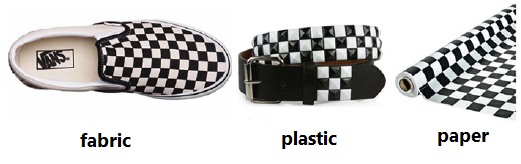
\includegraphics[width=0.8\textwidth]{ex1.png}
	\caption{Những đối tượng với chất liệu khác nhau nhưng bề mặt lại có texture giống nhau (đều là sọc ca-rô)}
    \label{fig:ex1}
\end{figure}

\begin{figure}[h!]
	\centering
	\captionsetup{width=0.9\textwidth}
	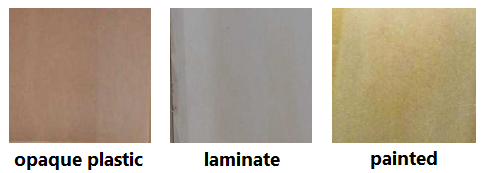
\includegraphics[width=0.8\textwidth]{ex2.png}
	\caption{Một ví dụ từ tập dữ liệu Open-Surface cho thấy bài toán này thách thức như thế nào}
    \label{fig:ex2}
\end{figure}


\chapter{Các công trình liên quan}
\ifpdf
    \graphicspath{{Chapter2/Chapter2Figs/PNG/}{Chapter2/Chapter2Figs/PDF/}{Chapter2/Chapter2Figs/}}
\else
    \graphicspath{{Chapter2/Chapter2Figs/EPS/}{Chapter2/Chapter2Figs/}}
\fi

\paragraph*{}
Từ khi ra đời, bài toán phân lớp vật liệu nhận được sự chú ý của rất nhiều nhóm nghiên cứu. Cùng với sự phát triển đó, rất nhiều tập dữ liệu mới cũng được xây dưng để giải quyết nhiều vấn đề khác nhau của bài toán. Hình \ref{fig:timeline} là tóm tắt các công trình nghiên cứu liên quan được công bố tại hội nghị CVPR (Conference on Computer Vision and Pattern Recognition) từ năm 2010 tới nay. Bên cạnh đó bảng 2.1 là tổng hợp một số tập dữ liệu được sử dụng.

\begin{figure}[h!]
	\centering
	\captionsetup{width=0.9\textwidth}
	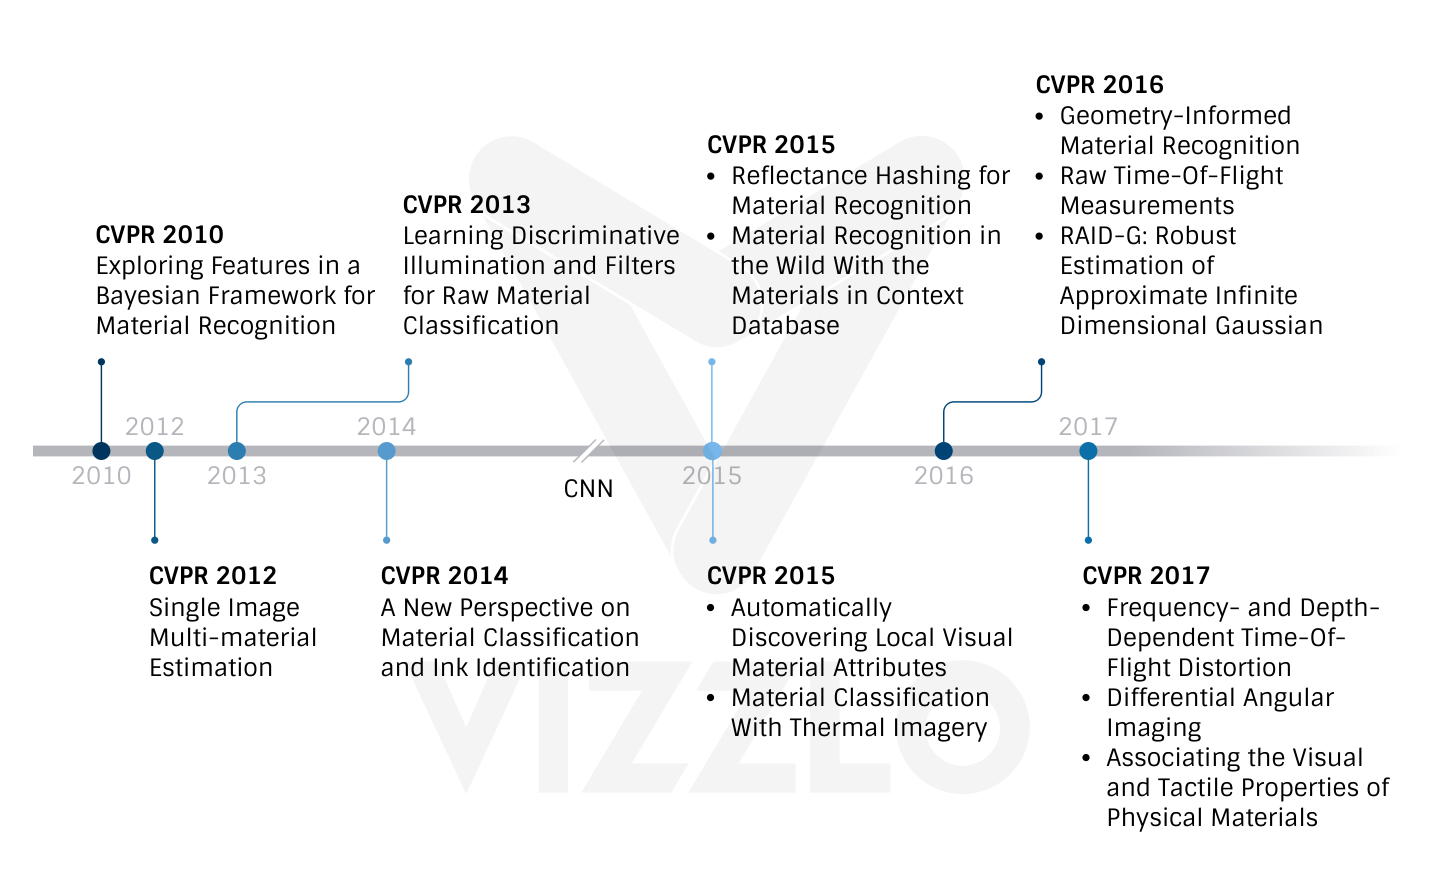
\includegraphics[width=1.0\textwidth]{timeline.png}
	\caption{Các nghiên cứu được công bố tại hội nghị CVPR qua các năm từ 2010 đến nay}
    \label{fig:timeline}
\end{figure}

\begin{table}
\label{tab:datasets}
\begin{center}
\resizebox{1.0\linewidth}{!}{
\begin{tabular}{l|l|l|l|l|l|l|l|l}
\toprule[1.0pt]
\head{Name}
& \head{Samples}
& \head{Classes}
& \head{Views}
& \head{Illumination}
& \head{In scene}
& \head{Scene image}
& \head{Camera parameters}
& \head{Year} \\
\midrule
CUReT \cite{dana1999reflectance} 				& 61	& 61	& 205	& 205 	& No	& No	& No	& 1999 	\\
KTH-TIPS \cite{hayman2004significance}			& 11	& 11	& 27	& 3		& No	& No	& No	& 2004	\\
UBO2014 \cite{weinmann2014material}				& 84	& 7		& 151	& 151	& No	& No	& No	& 2014	\\
Reflectance disk \cite{zhang2015reflectance}	& 190	& 19	& 3		& 3 	& No	& No	& Yes	& 2015	\\
4D Light-field \cite{wang20164d}				& 1200	& 12	& 1		& 1		& Yes	& No	& No	& 2016	\\
NISAR \cite{choe2016simultaneous} 				& 100	& 100	& 9		& 12	& No	& No	& No	& 2016	\\
GTOS \cite{xue2017differential} 				& 606	& 40	& 19	& 4		& Yes	& Yes	& Yes	& 2016 	\\
\bottomrule[1.0pt]
\end{tabular}}
\captionsetup{width=0.9\textwidth}
\caption{Một số tập dữ liệu được dùng cho phân lớp dữ liệu \cite{xue2017differential}}
\end{center}
\end{table}

\paragraph*{}
Một điểm chung có thể thấy, sau khi CNN bắt đầu được dùng nhiều trong Thị giác máy tính và chứng minh sự hiểu quả của chúng, số lượng và chất lượng của các nghiên cứu cũng tăng lên đáng kể (kết quả phân lớp rất chính xác, gần như bằng với khả năng đoán của con người), các tập dữ liệu được dùng cũng lớn hơn, đa dạng hơn.

\paragraph*{}
Có rất nhiều phương pháp khác nhau để giải quyết bài toán phân lớp vật liệu. Các phương pháp này có thể được chia thành hai nhóm chính: \textbf{Lab-based} và \textbf{Image-based}

\section{Lab-based methods}
\paragraph*{}
Đây là các phương pháp sử dụng chính các thông tin vật lý của đối tượng để phân lớp. Các thông tin vật lý có thể là độ đàn hồi (elasticity) \cite{davis2015visual}, sự thấm nước (water permeation) \cite{saponaro2015material}, phản ứng với ánh sáng (optical response) hay độ phản chiếu (reflectance) \cite{tanaka2017material}. Đây là các thông tin rất giá trị, vì vậy độ chính xác của các phương pháp này thường rất cao. Tuy nhiên quá trình xây dựng các bộ dữ liệu để thực hiện các phương pháp này rất kỳ công, đòi hỏi các thiết bị đặc biệt và một môi trường lý tưởng (vì vậy nên chúng có tên lab-based). Ví dụ, GelFabric \cite{yuan2017connecting} - tập dữ liệu ra đời năm 2016 chứa thông tin về chiều sâu và chỉ dùng để phân biệt các loại vải khác nhau; Ground Terrain in Outdoor Scenes (GTOS) \cite{xue2017differential} - năm 2016 dùng để lấy thông tin về các góc nhìn khác nhau cho cùng một mẫu trong dữ liệu; Reflectance Disk Database \cite{zhang2015reflectance} - năm 2015 với thông tin về sự phản chiếu của bề mặt. Thêm vào đó, các phương pháp khác nhau trong nhóm này thường đòi hỏi các thông tin vật lý khác nhau, chính vì thế tập dữ liệu của phương pháp khác nhau thường không thể dùng lại được. Ví dụ, một phương pháp dùng độ đàn hồi làm feature chính để phân lớp thì không thể dùng một tập dữ liệu chỉ có thông tin về độ thấm nước được. Vì vậy, các phương pháp đạt kết quả rất cao trên tập dữ liệu này có thể dễ dàng thất bại trên tập dữ liệu khác (hoặc không thể sử dụng trên dữ liệu khác vì thiếu thông tin). Hình \ref{fig:lab_based_1} và \ref{fig:lab_based_2} là hai ví dụ được lấy từ hai nghiên cứu năm 2017 và 2015 sử dụng các thông tin vật lý khác nhau (thông tin về chiều sâu, độ phản chiếu ánh sáng) để phân biệt các loại vật liệu. Cả hai đều đạt kết quả khá tốt trên những tập dữ liệu có đầy đủ thông tin trên \cite{tanaka2017material} \cite{zhang2015reflectance}

\begin{figure}[h!]
	\centering
	\captionsetup{width=0.9\textwidth}
	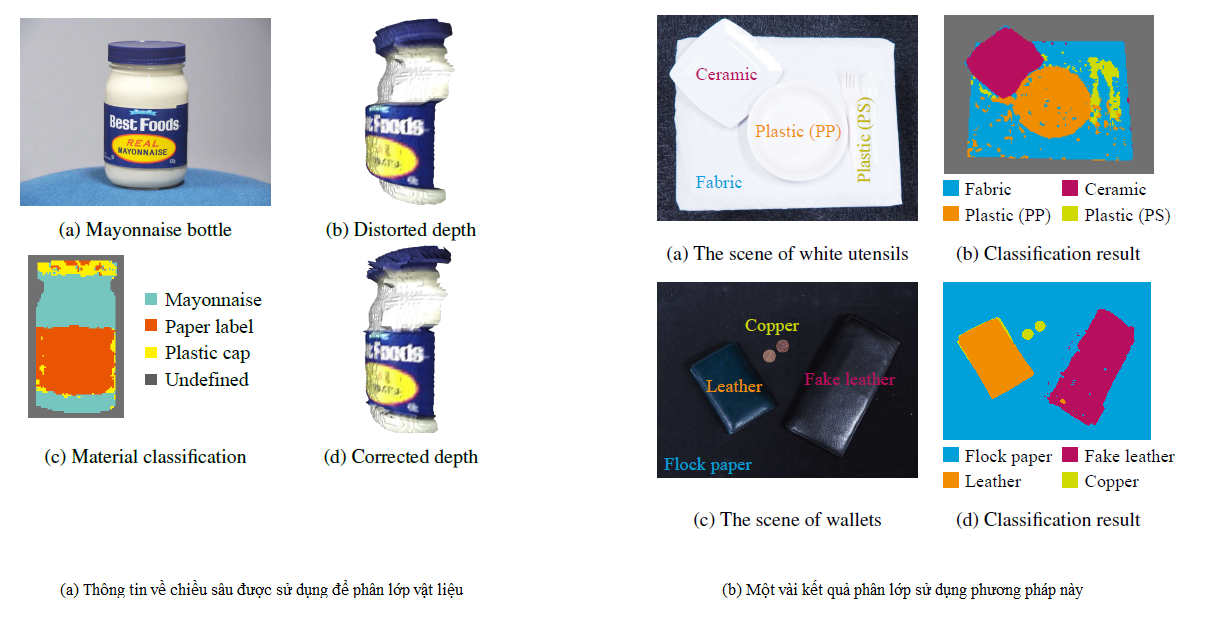
\includegraphics[width=1.0\textwidth]{lab_based_1.png}
	\caption{Thông tin về chiều sâu được dùng để phân lớp vật liệu trong một nghiên cứu 2017 \cite{tanaka2017material}}
    \label{fig:lab_based_1}
\end{figure}

\begin{figure}[h!]
	\centering
	\captionsetup{width=0.9\textwidth}
	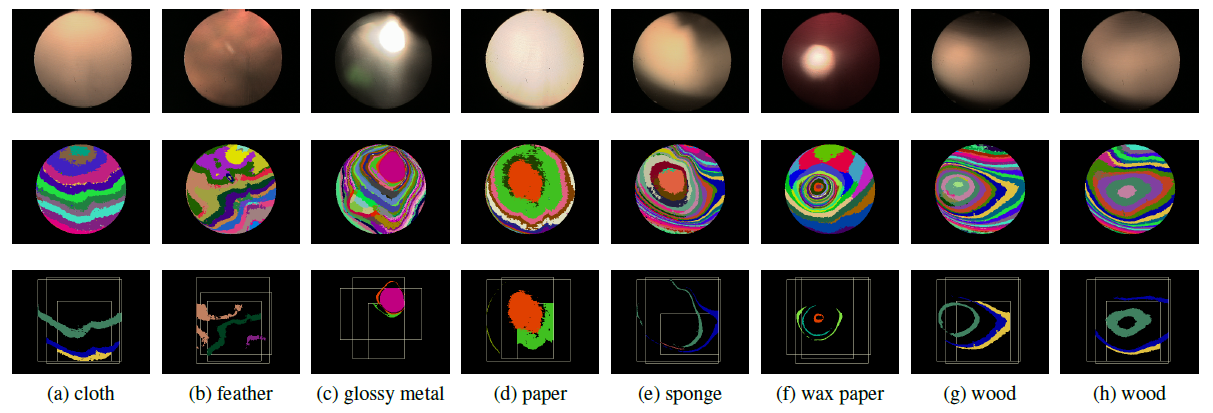
\includegraphics[width=1.0\textwidth]{lab_based_2.png}
	\caption{Thông tin về sự phản chiếu ánh sáng được dùng để phân lớp vật liệu trong một nghiên cứu 2015 \cite{zhang2015reflectance}}
    \label{fig:lab_based_2}
\end{figure}

\pagebreak

\section{Image-based methods}
\paragraph*{}
Ngược lại với các phương pháp Lab-base, Image-base là các phương pháp chỉ sử dụng ảnh màu RGB để phân lớp. Vì thế các tập dữ liệu cũng dễ dàng thu thập hơn, và các phương pháp này nếu có độ chính xác cao thì rất dễ để áp dụng vào thực tế. Dựa trên các thông tin trực quan (chẳng hạn như màu sắc) thông qua ảnh và thường dựa trên bài toán phân loại đối tượng để tìm ra vật liệu của ảnh (vì các phương pháp hiện tại dùng nhiều các mạng CNN được huấn luyện sẵn cho bài toán phân loại đối tượng để làm gốc), vấn đề chính của các hệ thống dùng phương pháp này chính là sự thiếu thông tin và vì thế chúng dễ dàng bị "lừa" bởi các ảnh có các đối tượng tương tự nhau nhưng lại khác nhau về chất liệu.
Hình \ref{fig:image_based_1} và \ref{fig:image_based_2} là hai ví dụ cho các phương pháp thuộc nhóm này được lấy từ các nghiên cứu năm 2010 \cite{liu2010exploring} và 2011 \cite{hu2011toward}. Trong những năm gần đây với sự phát triển của Deep Learning, các mạng CNN (Convolutional Neuron Network) được dùng thay thế cho các dạng local features này và nhiều nghiên cứu khác sử dụng các mạng CNN đã huấn luyện cho bài toán phân lớp đối tượng và đạt kết quả khá cao, tuy nhiên vẫn còn một số hạn chế như đã nêu bên trên. Nhóm tập trung giải quyết các hạn chế này và kế thừa các thành công từ CNN để cải thiện kết quả của bài toán.

\begin{figure}[h!]
	\centering
	\captionsetup{width=0.9\textwidth}
	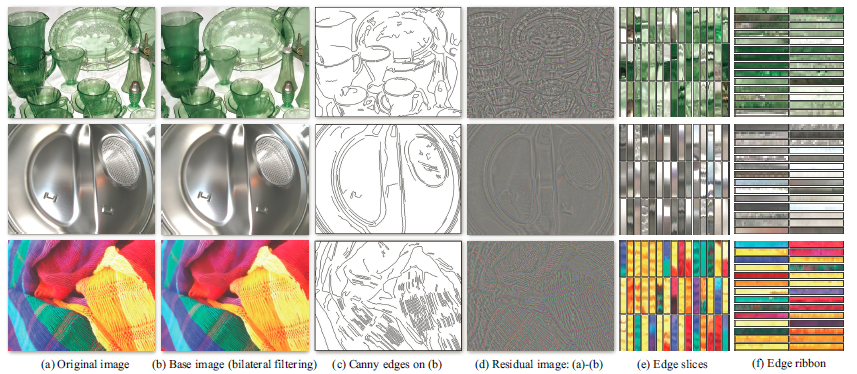
\includegraphics[width=1.0\textwidth]{image_based_1.png}
	\caption{Các local features (cạnh, \textit{micro structures}, SIFT - Scale-Invariant Feature Transform) được được dùng để phân lớp vật liệu trong một nghiên cứu 2010 \cite{liu2010exploring}}
    \label{fig:image_based_1}
\end{figure}

\begin{figure}[h!]
	\centering
	\captionsetup{width=0.9\textwidth}
	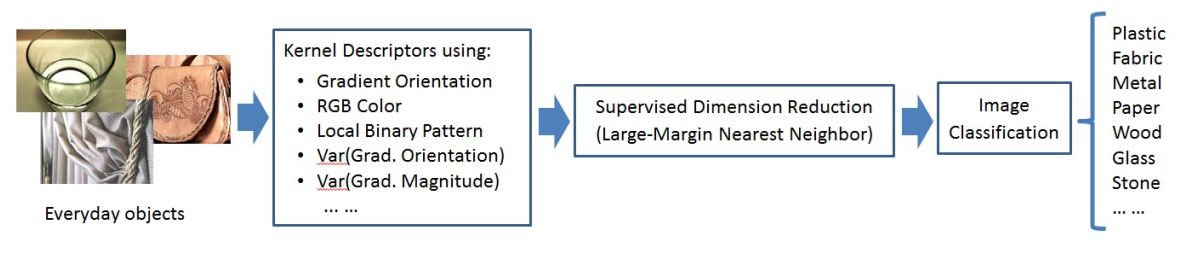
\includegraphics[width=1.0\textwidth]{image_based_2.png}
	\caption{Thông tin về gradient, màu sắc, local binary patterns được được dùng để phân lớp vật liệu trong một nghiên cứu 2011 \cite{hu2011toward}}
    \label{fig:image_based_2}
\end{figure}

\pagebreak
\paragraph*{}
Trong đề tài này, phương pháp mà nhóm sử dụng thuộc loại Image-based vì đối với lab-based, các tập dữ liệu sẽ được xậy dựng dựa trên phương pháp (đã có phương pháp X và xây dựng dữ liệu để phục vụ cho phương pháp X), cho nên các thông tin vật lý này dường như đã được sử dụng một cách triệt để nhất và nhóm sẽ có ít cơ hội hơn để cải tiến chúng. Ngoài ra, nhóm còn được thúc đẩy bởi một two-stream network (mạng với 2 nhánh chính) được dùng trên tập GTOS năm 2017\cite{xue2017differential}. Hình \ref{fig:dain} thể hiện ý tưởng chính của nghiên cứu này, sử dụng một hệ thống mạng CNN với hai nhánh đầu vào (một là ảnh gốc, hai là ảnh thể hiện thông tin khác nhau về góc nhìn (view-point) - hay được tác giả gọi là Differential Angular Image). Differential Angular Image được tạo thành bằng cách lấy hai ảnh của cùng một mẫu dữ liệu được chụp từ hai góc khác nhau (hai góc này chênh lệch không quá nhiều) trừ nhau (Hình \ref{fig:differential_angular}). 

\begin{figure}[h!]
	\centering
	\captionsetup{width=0.9\textwidth}
	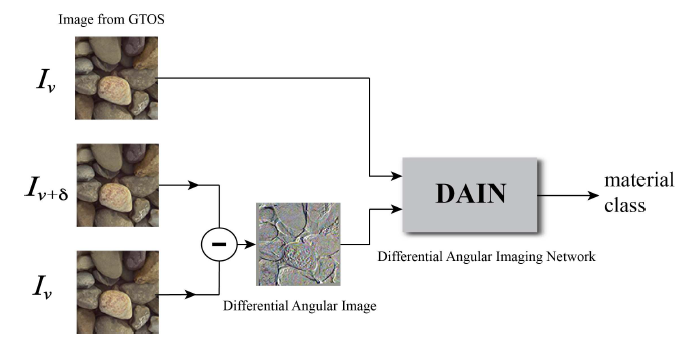
\includegraphics[width=1.0\textwidth]{dain.PNG}
	\caption{Two-stream network được dùng trên tập GTOS năm 2017 \cite{xue2017differential}}
    \label{fig:dain}
\end{figure}

\begin{figure}[h!]
	\centering
	\captionsetup{width=0.9\textwidth}
	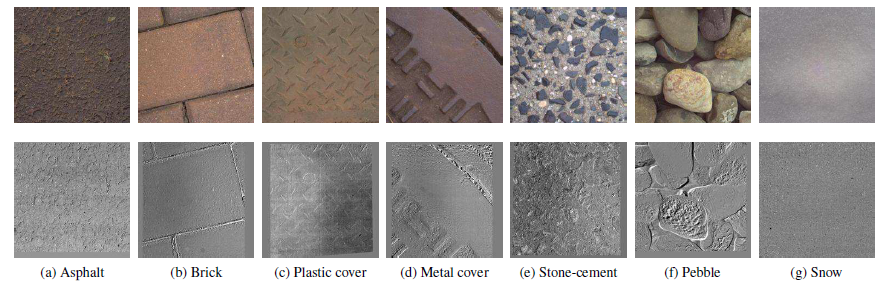
\includegraphics[width=1.0\textwidth]{diferential_angular.png}
	\caption{Differential Angular Image được tạo thành bằng cách lấy hai ảnh của cùng một mẫu dữ liệu được chụp từ hai góc khác nhau (hai góc này chênh lệch không quá nhiều) trừ nhau \cite{xue2017differential}}
    \label{fig:differential_angular}
\end{figure}

\begin{figure}[h!]
	\centering
	\captionsetup{width=0.9\textwidth}
	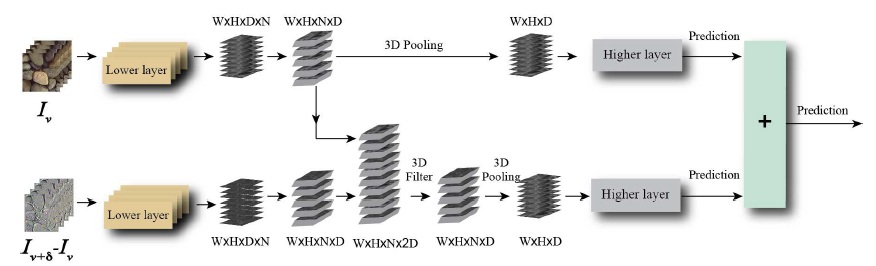
\includegraphics[width=1.0\textwidth]{dain_network.png}
	\caption{Cấu trúc bên trong của DAIN (Differential Angular Image Network) \cite{xue2017differential}}
    \label{fig:dain_network}
\end{figure}

\chapter{Cơ sở lý thuyết}
\ifpdf
    \graphicspath{{Chapter3/Chapter3Figs/PNG/}{Chapter3/Chapter3Figs/PDF/}{Chapter3/Chapter3Figs/}}
\else
    \graphicspath{{Chapter3/Chapter3Figs/EPS/}{Chapter3/Chapter3Figs/}}
\fi

\section{Support Vector Machines (SVMs)}
\paragraph*{}
Support Vector Machine là một trong những thuật toán học máy có giám sát (supervised learning) hiệu quả nhất. Được xây dựng dựa trên một nền tảng toán học vững chắc, SVM thường cho kết quả tốt trong nhiều bài toán mà không cần điều chỉnh quá nhiều. Tuy nhiên, cũng chính vì điều này mà nó thường được xem như một hộp đen (black box). Có nhiều thuật toán SVM khác nhau nên chúng thường được gọi chung là SVMs.Ở dạng chuẩn, SVM là thuật toán phân lớp nhị phân (binary classification). Từ dữ liệu huấn luyện, SVM xây dựng (learn) một siêu phẳng (hyperplane) để phân lớp (classify) tập dữ liệu thành hai lớp riêng biệt (Hình \ref{fig:svm}).

\begin{figure}[h!]
	\centering
	\captionsetup{width=0.8\textwidth}
	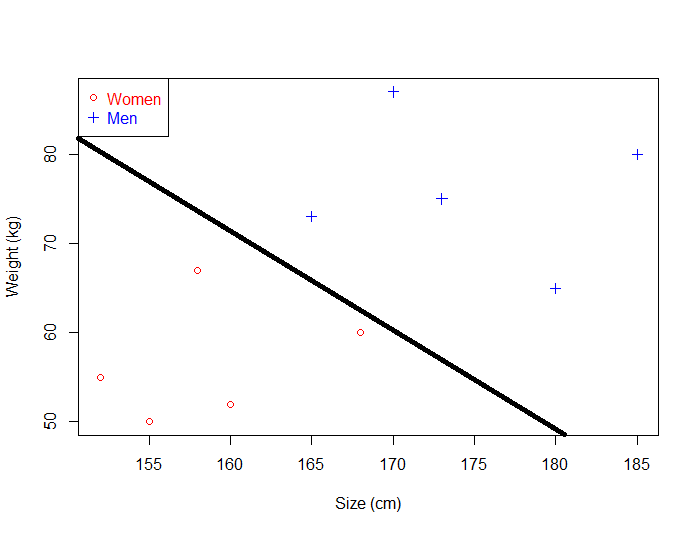
\includegraphics[width=0.9\textwidth]{svm.png}
	\caption{SVMs được dùng để phân lớp tập dữ liệu thành hai lớp phân biệt}
    \label{fig:svm}
\end{figure}

\paragraph*{}
SVMs là kết quả của một quá trình nghiên cứu xuyên suốt nhiều năm của rất nhiều người. Thuật toán SVM đầu tiên thuộc về Vladimir Vapnik năm 1963. Sau này, ông làm việc với Alexey Chervonenkis về cái được gọi là lý thuyết VC (VC theory - Vapnik–Chervonenkis theory), giải thích quá trình học từ góc nhìn của thống kê, và cả hai đều đóng góp rất nhiều cho SVM. Lịch sử chi tiết về SVM có thể được tìm thấy ở đây (http://www.svms.org/history.html).

\paragraph*{}
Trên thực tế, SVMs đã chứng minh được sự hiệu quả của mình trong rất nhiều lĩnh vực khác nhau: phân loại văn bản (text categorization), nhận diện ảnh (image recognition) và bioinformatics (Cristianini \& ShaweTaylor, 2000). Trong phần này, nhóm sẽ trình bày ý tưởng chính đằng sau và các khác niệm cơ bản được sử dụng trong SVM: vector, linear separability và hyperplanes.


\subsection{Các khái niệm liên quan}
\subsubsection*{Vector}
Vector là một đối tượng toán học có thể được biểu diễn bằng một mũi tên (\ref{fig:vector}). Vector được đặc trưng bởi hai thuộc tính chính là: độ dài (\textbf{vector magnitude}) và hướng (\textbf{vector direction}). Trong SVM, vector được dùng để biểu diễn cho các điểm dữ liệu (feature vector).
\begin{figure}[h!]
	\centering
	\captionsetup{width=0.8\textwidth}
	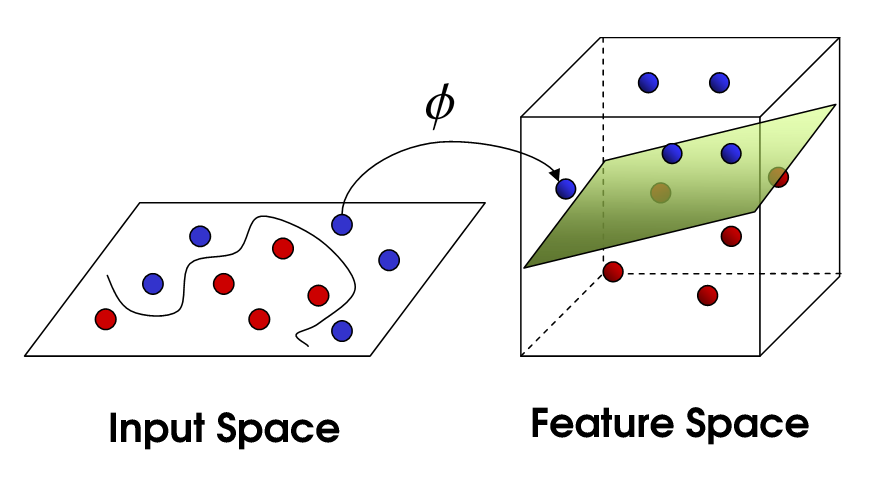
\includegraphics[width=0.9\textwidth]{svm_kernel.png}
	\caption{Magnitude của vector $\vec{OA}$ là độ dài đoạn OA}
    \label{fig:vector}
\end{figure}

\paragraph*{Vector magnitude}
Magnitude của một vector $x = (x_1, ..., x_n)$ (kí hiệu là $||x||$) là độ dài của vector x được tính dựa trên định lý Pythagorean (Hình \ref{fig:vector_mag}). Công thức \ref{eq:vector_mag} là công thức chung để tính magnitude của vector x được.
\begin{figure}[h!]
	\centering
	\captionsetup{width=0.8\textwidth}
	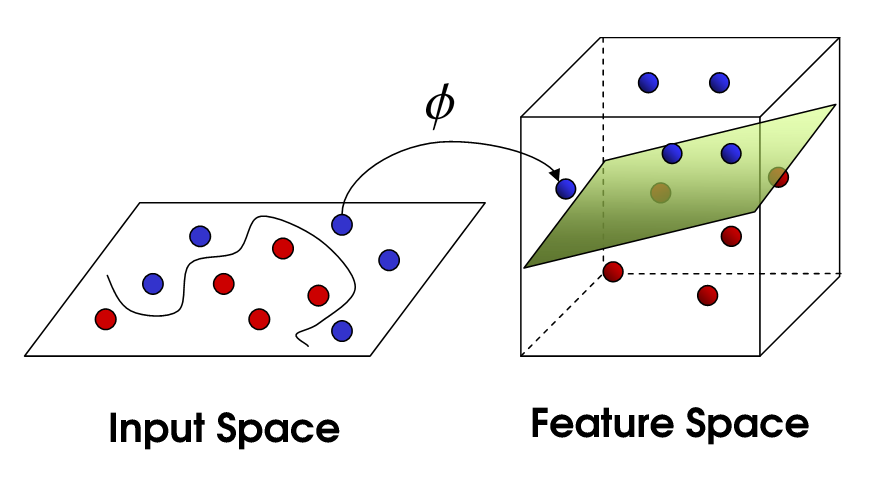
\includegraphics[width=0.9\textwidth]{svm_kernel.png}
	\caption{Magnitude của vector $\vec{OA}$ là độ dài đoạn OA}
    \label{fig:vector_mag}
\end{figure}
\begin{eqnarray}
\label{eq:vector_mag}
\hspace{1cm} ||x|| = \sqrt{x_1^2 + ... + x_n^2}
\end{eqnarray}
\paragraph*{Vector direction}
Hướng của vector $x = (x_1, ..., x_n)$ là một vector:
\begin{eqnarray}
\label{eq:vector_dir}
\hspace{1cm} w = (\frac{x_1}{||x||}, ..., \frac{x_n}{||x||})
\end{eqnarray}
Về mặt hình học, các giá trị của vector w $(w_1, ..., w_n)$ chính là giá trị cosin của các góc mà vector x lần lượt tạo với các trục tọa độ trong không gian của nó. Hình \ref{fig:vector_dir} thể hiện góc của vector x với hai trục tọa độ trong không gian hai chiều.

\begin{figure}[h!]
	\centering
	\captionsetup{width=0.8\textwidth}
	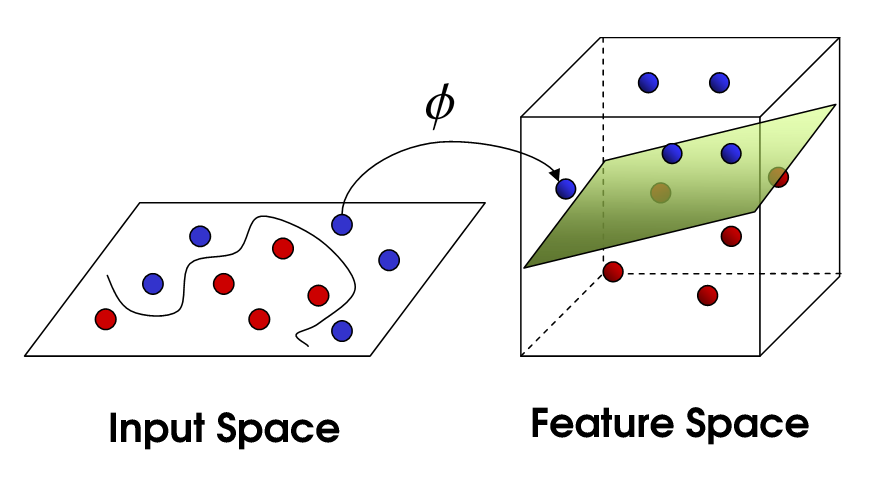
\includegraphics[width=0.9\textwidth]{svm_kernel.png}
	\caption{Hướng của vector u được thể hiện bởi góc mà u tạo với các trục tọa độ trong không gian của nó (Công thức \ref{eq:vector_mag_2})}
    \label{fig:vector_dir}
\end{figure}

\begin{eqnarray}
\label{eq:vector_mag_2}
\hspace{1cm} w = (\frac{u_1}{||u||}, \frac{u_2}{||u||}) = (\cos({\beta}), \cos({\alpha}))
\end{eqnarray}

\paragraph*{Tích vô hướng (dot product)}
Dot product là phép toán phổ biến được thực hiện trên hai vector và cho kết quả là một số thực (còn được gọi là scalar - vì vậy dot product còn có tên khác là scalar product). Dot product thể hiện mối quan hệ của hai vector. Về mặt hình học, dot product là tích của magnitude hai vector và cosin của góc tạo bởi hai vector này (Hình \ref{fig:dot_product}, công thức \ref{eq:dot_product_geometry}). Về mặt đại số, dot product có thể định nghĩa bằng công thức \ref{eq:dot_product_algebraic}. Dot product là phép toán cơ bản được dùng nhiều trong việc xây dựng SVM, đặc biệt là tìm hyperplane.
\begin{figure}[h!]
	\centering
	\captionsetup{width=0.8\textwidth}
	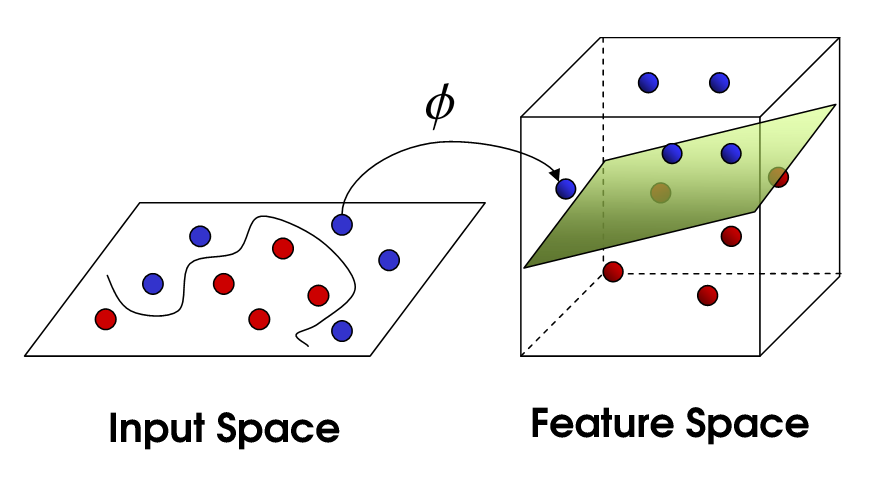
\includegraphics[width=0.9\textwidth]{svm_kernel.png}
	\caption{Hai vector x và y}
    \label{fig:vector_dir}
\end{figure}

\begin{eqnarray}
\label{eq:dot_product_geometry}
\hspace{1cm} x.y = ||x||||y||\cos({\theta})
\end{eqnarray}

\begin{eqnarray}
\label{eq:dot_product_algebraic}
\hspace{1cm} x.y = \sum_{i=1}^{n} (x_i.y_i)
\end{eqnarray}

\subsubsection*{Hyperplane (Siêu phẳng)}
Về mặt hình học, có thể hiểu hyperplane là một không gian con có số chiều nhỏ hơn không gian chứa nó. Trong không gian hai chiều, hyperplane là đường thẳng. Trong không gian ba chiều, hyperplane là một mặt phẳng (Hình \ref{fig:hyperplane}).
\begin{figure}[h!]
	\centering
	\captionsetup{width=0.8\textwidth}
	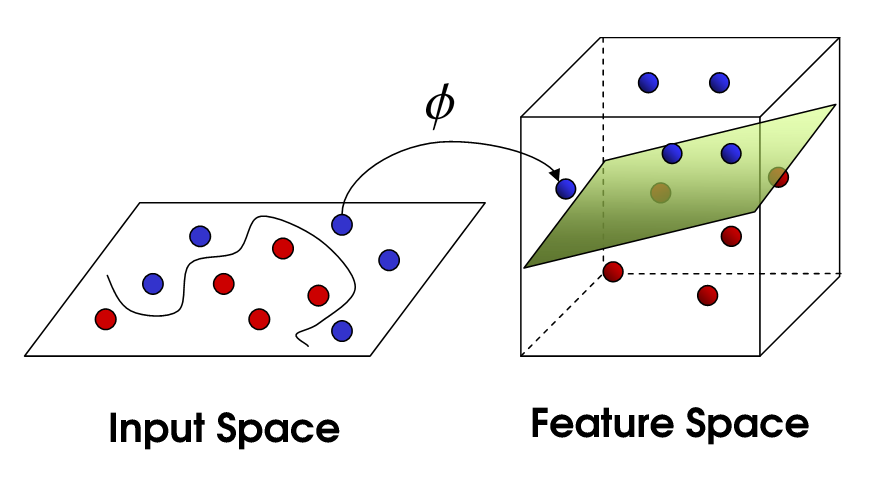
\includegraphics[width=0.9\textwidth]{svm_kernel.png}
	\caption{Hyperplane trong không gian hai chiều (đường thẳng) và ba chiều (mặt phẳng)}
    \label{fig:hyperplane}
\end{figure}
Với phương trình đường thẳng $y = ax + b$, ta có thể viết lại thành $x_2 = ax_1 + b$ hay $ax_1 - x_2 + b = 0$. Nếu đặt hai vector $x = (x_1, x_2)$ và $w = (a, -1)$ thì phương tình đường thẳng trở thành phương trình \ref{eq:hyperplane_eq}. Đây cũng chính là phương trình chung của hyperplane trên không gian bất kỳ.
\begin{eqnarray}
\label{eq:hyperplane_eq}
\hspace{1cm} wx + b = 0
\end{eqnarray}

\subsection{Ý tưởng chính của SVM}
Với bài toán phân lớp, mục tiêu của SVM là tìm một hyperplane "tối ưu" nhất để chia các điểm dữ liệu thành hai phần (binary classification). Để so sánh giữa hai hyperplane để chọn cái tốt hơn, chúng ta cần một thước đo. Ở đây chúng ta có hai tiêu chí để chọn một hyperplane, một là hyperplane này phải nằm giữa phân tách hai lớp dữ liệu và hai là hyperplane phải cách xa điểm dữ liệu nằm gần nó nhất (hay chính là bài toán maximize margin) (Hình \ref{margin}).
\linebreak
Cho tập dữ liệu $D = \{(x_i, y_i) | x_i \in \mathbb{R}, y_i \in[-1; 1]\}_{i=1}^m$. Chúng ta cần tìm một hyperplane $wx + b =0$ (hay chính là tìm w và b) sao cho M đạt giá trị lớn nhất với:
\begin{eqnarray}
\label{eq:hyperplane_eq}
\hspace{1cm} M = \min_{i=1}^m {y_i(\frac{wx + b}{||w||})}
\end{eqnarray}
Đây chính là bài toán maximize khoảng cách từ điểm dữ liệu gần hyperplane nhất đến hyperplane (maximize margin). Lưu ý ${y_i(\frac{wx + b}{||w||})}$ sẽ cho kết quả dương nếu điểm dữ liệu được phân lớp đúng và ngược lại âm nếu nó bị phân lớp sai.
Với bài toán tối ưu (Optimization Problem) này, để có thể sử dụng các phương pháp có sẳn từ toán học để giải, trước tiên chúng ta cần biến đổi nó một chút để về dạng đơn giản hơn. 
Bài toán chúng ta cần giải là:

\begin{center}
Maximize $M$ theo w và b
\linebreak
Sao cho $y_i(\frac{wx + b}{||w||}) >= M, i = 1, ..., m$
\end{center}

Đầu tiên vì ta có thể scale vector w và b một cách thích hợp mà không làm thay đổi phương trình hyperplane (ví dụ: hyperplane $5x_1 + x_2 + 1 = 0$ cũng có thể scale thành $10x_1 + 2x_2 + 2 = 0$), nên ta có thể đặt $F = \min_{i=1}^m {y_i(wx + b)} = 1 $ mà không ảnh hướng đến kết quả bài toán. Khi đó bài toán được viết lại:

\begin{center}
Maximize $\frac{1}{||w||}$ theo w và b
\linebreak
Sao cho $y_i({wx + b}) >= 1, i = 1, ..., m$
\end{center}

Sau khi dùng các phương pháp toán học đã có sẵn để giải quyết bài toán tối ưu này, chúng ta sẽ tìm được hyperplane phân tách các điểm dữ liệu thành hai lớp, với dữ liệu mới ta chỉ cần thay vào phương trình của hyperplane và quyết định xem nó thuộc lớp nào.

\begin{figure}[h!]
	\centering
	\captionsetup{width=0.8\textwidth}
	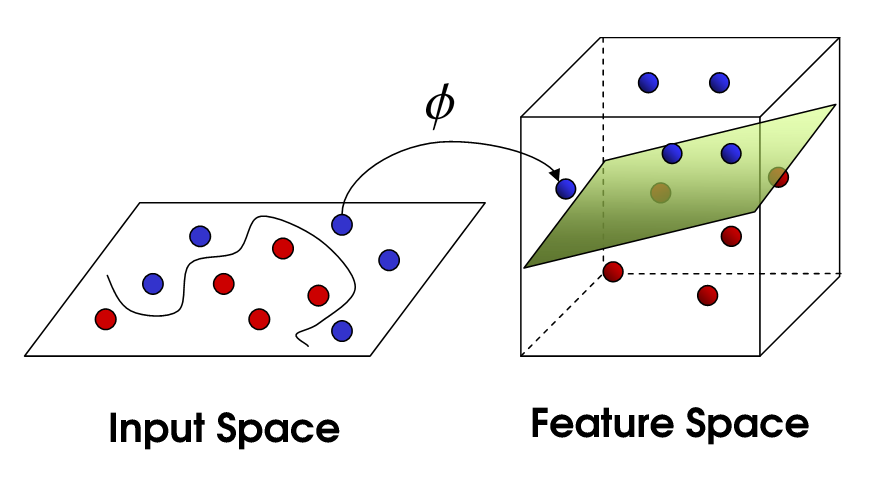
\includegraphics[width=0.9\textwidth]{svm_kernel.png}
	\caption{Dữ liệu được ánh xạ lên không gian cao hơn trước khi các bộ phân lớp được học}
    \label{fig:svm_kernel}
\end{figure}

\paragraph*{}
Tuy nhiên dữ liệu thực tế rất phức tạp và đan xen lẫn nhau khiến chúng ta không thể tìm được hyperplane nào có thể phân tách chúng trên không gian hiện tại, khi đó một phép ánh xạ sẽ được thực hiện để đưa các điểm dữ liệu này vào không gian với số chiều lớn hơn và hy vọng tìm được một hyperplane ở không gian này. Hình \ref{fig:svm_kernel} là ví dụ cho phép ánh xạ này. Nếu chúng ta xem các chấm màu xanh và đỏ là những quả bong bóng, trong hình bên trái, các quả bóng này được đặt trên bàn, nếu chúng phân bố không quá đan xen vào nhau, ta có thể dùng một cây que dài để chia các quả bóng thành hai tập xanh và đỏ mà không động đến các quả bóng. Lúc này, khi đưa một quả bóng mới đặt lên mặt bàn, bằng cách xác định nó nằm bên phía nào của cây que, ta có thể dự đoán màu sắc của quả bóng đó. Các quả bóng tượng trưng cho các điểm dữ liệu, màu xanh và đỏ tượng trưng cho 2 lớp. Cái bàn tượng trưng cho một mặt phẳng. Cây que tượng trưng cho một siêu phẳng đơn giản đó là một đường thẳng. Tuy nhiên khi các quả bóng nằm đan xen nhau trên bàn (dữ liệu phức tạp hơn), lúc này không thể dùng cái que để phân tách chúng, để làm được điều này chúng ta cần hất các quả bóng bay lên (chính là phép ánh xạ), từ đó có thể sử dụng một tờ giấy để phân tách chúng (tờ giấy chính là siêu phẳng). Trên thực tế, SVMs thực hiện ánh xạ bằng việc sử dụng các kernel thích hợp. Việc lựa chọn kernel với các tham số thích hợp sẽ giúp SVM học được các bộ phân lớp tốt hơn trên những tập dữ liệu khác nhau

\subsection*{Margin}
Margin là một thuật ngữ quan trọng trong SVM chỉ khoảng cách giữa siêu phẳng đến 2 điểm dữ liệu gần nhất tương ứng với các phân lớp (\ref{fig:svm_margin}). Để có được bộ phân lớp tốt nhất, SVM cố gắng maximize margin này, từ đó thu được một siêu phẳng tạo khoảng cách xa nhất với hai lớp, nhờ vậy có thể giảm thiểu việc phân lớp sai (misclassification) đối với điểm dữ liệu mới đưa vào.

\begin{figure}[h!]
	\centering
	\captionsetup{width=0.8\textwidth}
	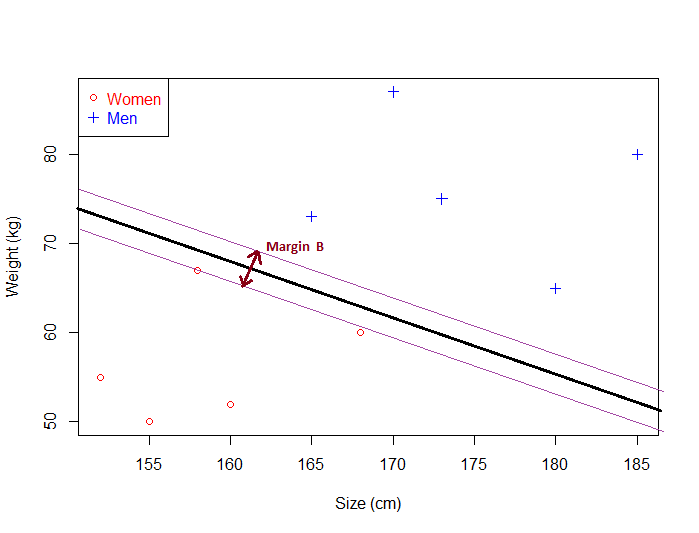
\includegraphics[width=0.7\textwidth]{svm_margin.png}
	\caption{Margin được maximize để giảm thiểu phân lớp sai cho dữ liệu mới}
    \label{fig:svm_margin}
\end{figure}

\paragraph*{}
Trong luận văn này, nhóm sử dụng SVM để huấn luyến các bộ phân lớp dựa trên các đặc trưng rút trích từ ảnh để phân lớp các loại vật liệu.

\section{Neural Network}

Neural Network là một loại hệ thống máy tính đặc biệt \cite{sampson1987parallel}, được lấy cảm hứng từ cấu trúc não của con người. Một tế bào trong não người được gọi là nơron có hai thành phần chính: Axons và Dendrites. Những tế bào thần kinh này hoạt động bằng cách xử lý các tín hiệu điện. Dựa trên tín hiệu nhận được thông qua Dendrites, Axons thực hiện mã hóa thần kinh (Neural coding) \cite{thorpe1990spike}, sau đó được phân phối tín hiệu này qua các Neurons và có thể được coi là đầu ra của hệ thần kinh. Axon của một Neuron được kết nối với Dendrites của Neurons khác, cứ như vậy các Neurons liên kết với nhau và hình thành Neurons Network trong não người (Hình \ref{fig:neuron}).

\begin{figure}[h!]
	\centering
	\captionsetup{width=0.7\textwidth}
	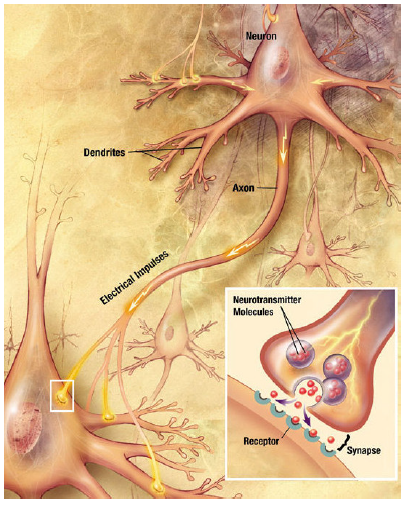
\includegraphics[width=0.5\textwidth]{neurons_network.PNG}
	\caption{Tín hiệu được truyền từ Axons của một neuron đến Dendrites của neuron tiếp theo}
    \label{fig:neuron}
\end{figure}

Với các tiến bộ trong khoa học máy tính, hiện nay chúng ta đã có thể phát triển hệ thống mạng hoạt dựa trên cách lan truyền tín hiệu của các nerouns trong hệ thần kinh. Thành phân cơ bản của hệ thống này là các nút (node) tương tác với nhau thông qua các trọng số và hàm lan truyền. Các node tương tự như các nerouns trong não. Một mạng neroun là sự kết hợp của nhiều layer của các node. Các layers được chia thành input layer, output layer và intermediate layer (còn được gọi là hidden layer). Đầu ra của mỗi node được tính toán thông qua hàm kích hoạt (activation function). Mỗi node gắn với mỗi giá trị trọng số (weight) và độ lệch (basis) riêng, hai giá trị. Trong nhiều trường hợp, mạng neroun là một hệ thống thích ứng (adaptive system) tự thay đổi cấu trúc của mình (các trọng số) dựa trên các thông tin bên ngoài hay bên trong đi qua mạng trong quá trình học.

\begin{figure}[h!]
	\centering
	\captionsetup{width=0.7\textwidth}
	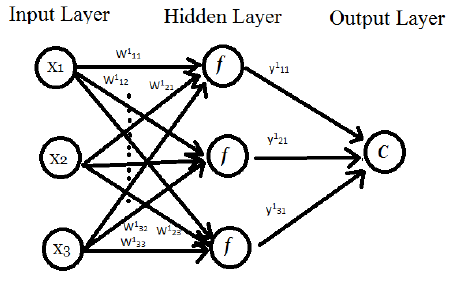
\includegraphics[width=0.5\textwidth]{single_layer_network.PNG}
	\caption{Cấu trúc của một Feedforward Perceptron Neural Network đơn giản.}
    \label{fig:simple_network}
\end{figure}

Hình \ref{fig:simple_network} là cấu trúc của một mạng neural đơn giản. Thuật ngữ "Feedforward" được dùng để chỉ cách dữ liệu đi qua mạng, trong trường hợp này dữ liệu chỉ đi qua mạng một chiều. Layer đầu tiên lấy các thông tin từ đầu vào, được gọi là input layer. Khi các giá trị đầu vào được truyền qua input layer, mỗi node sẽ tính toán giá trị output thông qua weights và biases, sau đó truyền output này tới hidden layer. Tại đây, các nodes dùng activation function để tính toán đầu ra rồi tiếp tục truyền tới layer cuối. Layer này được gọi là output layer, tính toán tất cả các "score" từ giá trị lan truyền từ layer trước. Với bài toán phân lớp, kết quả cuối cùng chính là lớp với giá trị "score" cao nhất sau khi qua output layer.

Giá trị đầu ra của mỗi node trong mạng được tính toán theo phương trình \ref{eq:simple_network}. Trong đó, $y_{j}$ là giá trị đầu ra của node thứ j của layer hiện tại, n là số lượng node của layer trước truyền thông tin vào node hiện tại, $f$ là hàm kích hoạt của node, $w_{mn}$ là trọng số được truyền từ node thứ m của layer trước đến node thứ n của layer hiện tại, $b_j$ là bias của node hiện tại (đang cần tính đầu ra)

\begin{eqnarray}
\label{eq:simple_network}
\hspace{1cm} y_{j} = f(\sum_{i=1}^{n} {w_{ij}x_i} + b_j)
\end{eqnarray}

Node đầu ra C sẽ nhận giá trị của các $y_j$ sau đó chọn lớp có score lớn nhất là output cuối cùng. Phương trình \ref{eq:y1}, \ref{eq:y2} và \ref{eq:y3} là cách tính giá trị đầu ra của từng node trong hidden layer
\begin{eqnarray}
\label{eq:y1}
\hspace{1cm} y_{1} = f(w_{11}x_1 + w_{21}x_2 + w_{31}x_3  + b_1)\\
\label{eq:y2}
\hspace{1cm} y_{2} = f(w_{12}x_1 + w_{22}x_2 + w_{32}x_3  + b_2)\\
\label{eq:y3}
\hspace{1cm} y_{3} = f(w_{13}x_1 + w_{23}x_2 + w_{33}x_3  + b_3)
\end{eqnarray}

Một hệ thống mạng neural với khả năng học tập hạn chế đã được phát triển trong công trình của Lugar và Stubble \cite{luger2005artificial} và được gọi là Perceptron. Mỗi node sẽ có đầu ra là 0 hoặc 1 được tính toán dựa trên một giá trị ngưỡng đặc biệt. Mạng neural này sẽ được học trên một tập dữ liệu huấn luyện. Mỗi mẫu trong tập huấn luyện gốm các giá trị đầu vào và giá trị đầu ra mong muốn tương ứng với nó. Các giá trị đầu vào được truyền vào input layer, đi qua mạng neural và cho một giá trị đầu ra (ở đây là 0 hoặc 1). Nếu giá trị đầu ra của mạng không giống với giá trị đầu ra mong muốn ban đầu thì giá trị các weights và thresholds sẽ được điều chỉnh để có kết quả tốt hơn. Hình \ref{fig:change_weights} là một cách thay đổi weights và thresholds để có kết quả tốt hơn.

\begin{figure}[h!]
	\centering
	\captionsetup{width=0.7\textwidth}
	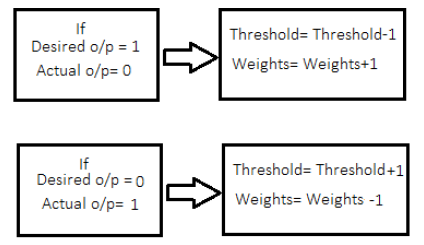
\includegraphics[width=0.5\textwidth]{change_weights.PNG}
	\caption{Một trong những cách đơn giản thay đổi weights và thresholds của một node để có kết quả tốt hơn}
    \label{fig:change_weights}
\end{figure}

Perceptron sau đó được phát triển thành mạng với nhiều hidden layer (multilayer). Cấu trúc này được học dựa trên thuật toán lan truyền ngược (backpropagation) \cite{sampson1987parallel}. Thuật toán này tuân theo quy tắc delta [\ref{widrow1960adaptive} để tính toán độ lỗi tại nút đầu ra. Độ lỗi của nút cuối cùng trong mạng (output node) được lan truyền ngược qua mạng sau mỗi lần huấn luyện, giá trị các weights sẽ 	được cập nhật dựa trên hàm lỗi. Cách học này còn được gọi là gradient descent. 
Giá trị đầu ra của một node phụ thuộc vào hàm kích hoạt và trong mạng lan truyền ngược là một hàm sigmoid (Phương trình \ref{sigmoid_function}) với $f_{j} = \sum_{i=1}^{n} {w_{ij}x_i}$

\begin{eqnarray}
	\label{eq:sigmoid_function}
	\hspace{1cm} \sigma(f_x) = \frac{1}{1 + e^{-f_x}}
\end{eqnarray}

Hàm sigmoid áp dụng cho tất cả các node trừ các input node và giá trị đầu ra được giới hạn trong khoảng [0,1].

\section{Convolutional Neural Networks (CNNs)}
Convolutional Neural Networks (CNNs) là một loại Neural Network đặc biệt. Nguyên tắt hoạt động của CNNs tương tự như một Neural Network bình thường: lấy input tại input layer, truyền giá trị này qua các hidden layer, dùng activation function tính toán giá trị đầu ra tại mỗi node. Score tại các node ở layer cuối (output layer) được lan truyền ngược và các trọng số của mạng được cập nhật sau mỗi lần huấn luyện. Trong thực tế, CNNs khó huấn luyến hơn các Neural Network bình thường do sự phức tạp của nó.Nhưng điều gì khiến CNNs đặc biệt hiệu quả trong các vấn đề của Thị Giác Máy Tính? Hãy cùng tìm hiểu bên dưới.

Các Neural Network bình thường không thích ứng tốt với các ảnh đầu vào khác nhau. Với ảnh đầu vào 32x32 RGB, input layer sẽ có $32*32*3 = 3072$ weights. Nhưng trên thực tế, kích thước của ảnh đầu vào lớn hơn nhiều, cho một ảnh với kích thước 600x300 RGB, sẽ có tới $600*300*3 = 540000$ weights chỉ tính input layer - một con số không hề nhỏ! Để khắc phục điều này nhận cả bức ảnh làm đầu vào. Năm 2012, CNNs bắt đầu nhận được sự chú ý của nhiều nhà nghiên cứu trong lĩnh vực phân lớp ảnh khi Alex Krizhevsky thắng giải trong cuộc thi của Imagenet bằng việc thiết kế một mạng CNN và giảm độ lỗi trong việc phân lớp đối tượng từ 26.2\% xuống còn 15.3\% \cite{krizhevsky2012imagenet}. CNN tận dụng lợi thế của bất kỳ cấu trúc đầu vào nào thể hiện mối tương quan không gian (chẳng hạn như hình ảnh) và sắp xếp các neural theo không gian này. Sự sắp xếp này cho phép thông tin đi qua mạng hiệu quả và giảm đáng kể số lượng tham số của mạng. Cấu trúc của một mạng CNN gồm nhiều phần khác nhau: Convolutional Layer, Pooling Layer, Rectied Linear Unit hoặc ReLU Layer và Fully Connected Layer. Một trong những kiến trúc CNN cơ bản (LeNet-5) \cite{lecun1998gradient} dùng cho nhận diện chữ viết được thể hiện trong hình \ref{fig:lenet_5}

\begin{figure}[h!]
	\centering
	\captionsetup{width=0.7\textwidth}
	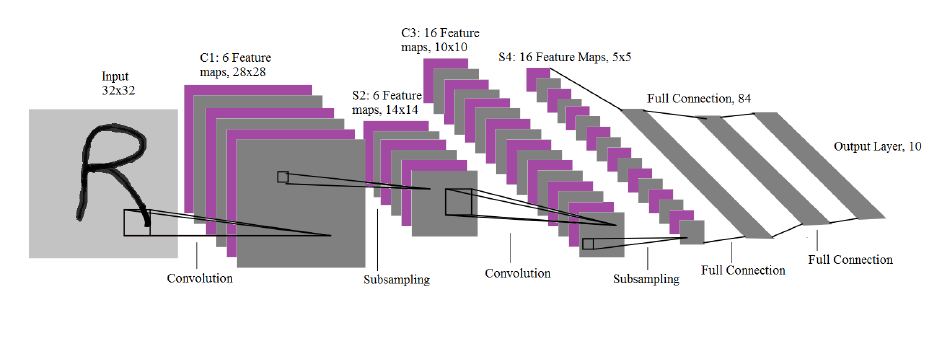
\includegraphics[width=1.0\textwidth]{lenet_5.PNG}
	\caption{Cấu trúc mạng LeNet-5, một mạng CNN dùng cho nhận diện chữ viết}
    \label{fig:lenet_5}
\end{figure}

\subsection*{Convolutional layer}
Convolutional layer là thành phần chính thực hiện hầu hết các tính toán trong một mạng CNN, Mỗi convolutional layer chứa một tập các filters (hay kernels) với kích thước ứng với các weights và biases. Trong quá trình lan truyền của một mạng CNN, mỗi kernel trượt qua tất cả các vùng của ảnh đầu vào và thực hiện phép toán dot product trên mỗi vùng đó. Mỗi kernel rút trích các đặc trưng khác nhau từ ảnh. Các phép toán này làm giảm dần số chiều (kích thước) của đầu vào nhưng cũng làm tăng độ sâu của mạng.

Ba tham số quyết định đầu ra của một convolutional layer bao gồm: depth, stride và zero-padding. \textbf{Depth} thay đổi đầu ra của convolutional layer dựa vào số lượng kernel của layer đó. Số lượng kernel càng lớn thì đầu ra của layer sẽ càng "sâu". \textbf{Stride} là tham số thể hiện bước nhảy của kernel khi trượt trên ảnh để thực hiện dot product. Nếu stride có giá trị là 1 thì kernel se trượt một pixel sau mỗi phép dot product. Bằng cách này, stride sẽ quyết định kích thước của đầu ra. \textbf{Zero-padding} cũng ảnh hưởng đến kích thước của đầu ra thông qua việc thêm 0 vào các cạnh của ảnh hay ma trận đầu vào. 

\begin{figure}[h!]
	\centering
	\captionsetup{width=0.7\textwidth}
	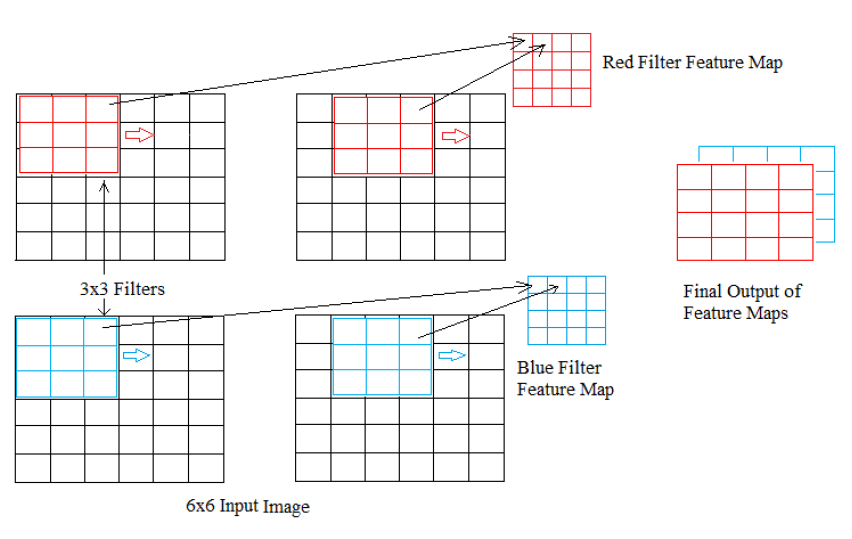
\includegraphics[width=1.0\textwidth]{filters.PNG}
	\caption{Hai filter 3x3 được dùng để tính toán hai 4x4 2D feature map từ một ma trận đầu vào 6x6}
    \label{fig:filters}
\end{figure}

Hình \ref{fig:filters} thể hiển quá trình tính toán của một convolutional layer sử dụng 2 filters 3x3 cho ma trận đầu vào 6x6 (không dùng zero-padding). Sau khi các phép toán dot product hoàn thành, kết quả đầu ra của layer này là hai 2D feature map 4x4 (hay có thể nói đầu ra có kích thước 4x4x2). Đây chính là ví dụ cho việc giảm kích thước đầu vào nhưng tăng chiều sâu của layer trong mạng CNN. Một cách tổng quát, với ma trận đầu vào kích thước NxN đi qua một convolutional layer với Y filters MxM (stride = 1 và không dùng zero-padding) thì đầu ra có kích thước (N - M + 1) X (N - M + 1) X Y

\subsection*{Pooling Layer}
Là một loại layer quan trọng khác trong CNN, pooling layer thường được dùng ở giữa hai convolutional layers. Pooling layer được dùng để giảm kích thước của ma trận đầu vào (vì vấy nó còn có tên khác là downsampling layer). Kiểu pooling layer phổ biến nhất là max pooling layer, thường sử dụng với filter có kích thước 2x2 và stride = 2 pixels. Hình \ref{fig:max_pooling} cho thấy tác dụng của layer này, giảm kích thước ma trân đầu vào từ 4x4 xuống còn 2x2.

\begin{figure}[h!]
	\centering
	\captionsetup{width=0.7\textwidth}
	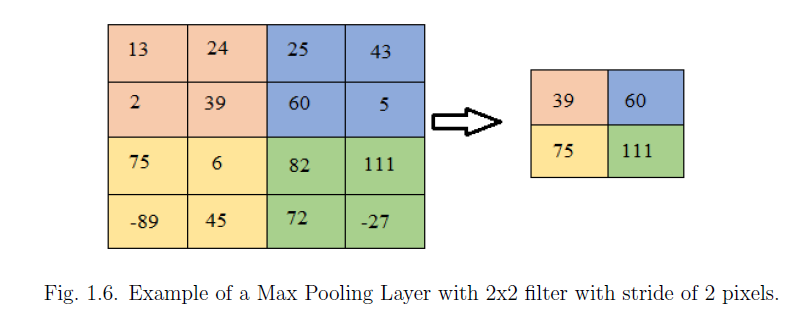
\includegraphics[width=1.0\textwidth]{max_pooling.PNG}
	\caption{Một max pooling layer với filter 2x2 và stride = 2 pixels}
    \label{fig:max_pooling}
\end{figure}

Những phương pháp gần đây thường không dùng pooling layer ở giữa hai convolutional layer. Thay vào đó, để đạt được tác dụng tương tự pooling layer (giảm kích thước), stride của convolutional layer thường được dùng với giá trị cao hơn \ref{springenberg2014striving}.

\subsection*{ReLU (Rectied Linear Unit) Layer}
Rectied Linear Unit hay ReLU layer thường được dùng sau convolutional layer và trước pooling layer. Thực nghiệm cho thấy layer này được dùng để tăng hiệu quả tính toán của mạng CNN [16].
ReLU layer không thay đổi kích thước của ma trận đầu vào. Trong ví dụ Hình \ref{fig:relu}, layer này sử dụng hàm $f(x) = max(0, x)$ để thay đổi tất cả các giá trị âm thành 0.

\begin{figure}[h!]
	\centering
	\captionsetup{width=0.7\textwidth}
	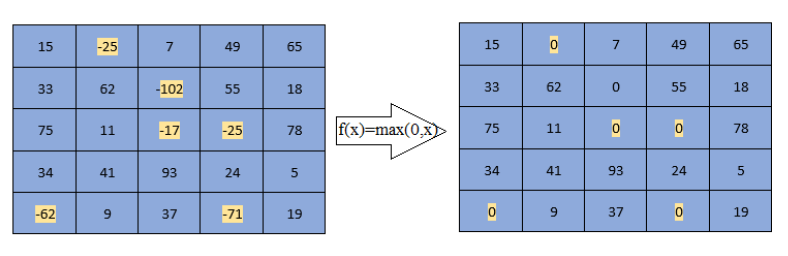
\includegraphics[width=1.0\textwidth]{relu.PNG}
	\caption{ReLU layer sử dụng hàm $f(x) = max(0, x)$ để thay đổi tất cả các giá trị âm thành 0}
    \label{fig:relu}
\end{figure}

\subsection*{Fully Connected Layer}
Fully connected layer được dùng như layer cuối cùng của một mạng CNN (output layer). Tại đây, mỗi node trong layer trước liên kết với tất cả các node của layer tiếp theo, Layer này được dùng để chuyển đổi feature map từ layer trước thành classification score.

\section{Transfer Learning}
Với bài toán phân lớp ảnh, để đạt kết quả tốt đòi hỏi một cấu trúc mạng thích hợp, điều này phụ thuộc nhiều vào tập dữ liệu huấn luyện. Trong thực tế, dữ liệu huấn luyện rất lớn và đa dạng. Một cấu trúc mạng tốt có thể học được khối lượng dữ liệu lớn thường rất phức tạp và đòi hỏi khá nhiều về phần cứng để thực hiện huấn luyện. Alexnet \cite{krizhevsky2012imagenet} sử dụng hơn 1.2 triệu ảnh thuộc 1000 lớp khác nhau để huấn luyện trên hai GTX 580 3GB GPUs trong gần một tuần.

Với các bài toán trên tập dữ liệu khác, kỹ thuật transfer learning được dùng để sử dụng lại các mạng phức tạp đã được huấn luyện sẵn này, và chỉ huấn luyện lại một phần nhỏ để thích hợp với bài toán mới. Cách tiếp cân này đã được được rất nhiều kết quả tốt trong nhiều bài toán phân lớp trên những tập dữ liệu khác nhau.

Một cách đơn giản nhưng hiểu quả để áp dụng kỹ thuật này là sử dụng lại toàn bộ một mạng CNN được train trên tập dữ liệu lớn, thay layer cuối cùng bằng một Softmax Regression nhưng với số lượng units bằng với số lượng class ở bộ cơ sở dữ liệu mới và chỉ huấn luyện lại tham số cho layer này để giảm thiểu chi phí tính toán và thời gian

Ngoài ra, chúng ta cũng có thể sử dụng feature map ở những layer gần cuối (fully connected layers) rút ra từ các mạng được huấn luyện sẵn như một feature (deep feature) và sử dụng các thuật toán máy học như SVMs (Support Vector Machines) để huấn luyện các bộ phân lớp cho bài toán mới.
\chapter{Phương pháp đề xuất}
\ifpdf
    \graphicspath{{Chapter4/Chapter4Figs/PNG/}{Chapter4/Chapter4Figs/PDF/}{Chapter4/Chapter4Figs/}}
\else
    \graphicspath{{Chapter4/Chapter4Figs/EPS/}{Chapter4/Chapter4Figs/}}
\fi

Như đã đề cập bên trên, các phương pháp phân lớp vật liệu dựa trên ảnh RGB thường dựa trên việc phân lớp đối tượng để phân loại vật liệu của chúng, điều này khiến những hệ thống này dễ phân loại sai khi những đối tượng có hình dạng hoặc texture tương tự nhau (Hình \ref{fig:shape} và \ref{fig:texture}). Nhóm đề xuất phương pháp kết hợp deep feature rút trích từ một CNN được huấn luyện sẵn (transfer learning) với các handcrafted features thích hợp trên những tập dữ liệu khác nhau (thể hiện thông tin về hình dạng và texture) để giải quyết sự nhầm lần nãy và cải thiện kết quả phân lớp (Hình \ref{fig:main_idea}). 

\begin{figure}[h!]
	\centering
	\captionsetup{width=0.75\textwidth}
	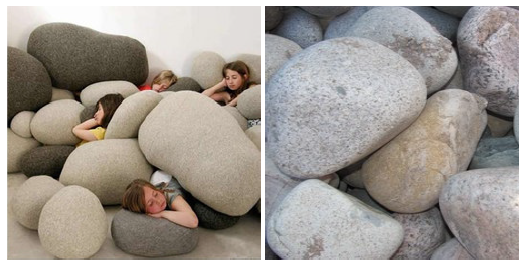
\includegraphics[width=0.8\textwidth]{shape.png}
	\caption{Các đối tượng chính của hai ảnh đều có hình dạng giống nhau và có thể bị nhầm lần cả hai đều là đá}
    \label{fig:shape}
\end{figure}

\begin{figure}[h!]
	\centering
	\captionsetup{width=0.75\textwidth}
	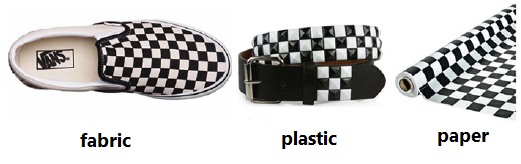
\includegraphics[width=0.8\textwidth]{texture.png}
	\caption{Các đối tượng có hình dạng khác nhau được làm từ vật liệu khác nhau nhưng lại giống nhau về texture (đều là sọc caro)}
    \label{fig:texture}
\end{figure}

\begin{figure}[h!]
	\centering
	\captionsetup{width=0.7\textwidth}
	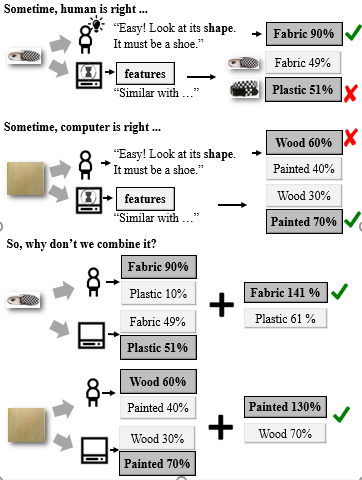
\includegraphics[width=1.0\textwidth]{main_idea.PNG}
	\caption{Deep features rút trích từ một mạng CNN đã được huấn luyện sẵn thê hiện cho cách con người học, kết hợp chúng với các handcrafted features thích hợp có thể giúp cải thiện kết quả phân lớp}
    \label{fig:main_idea}
\end{figure}

\section{Mô hình 1: kết hợp probability predictions (posfusion)}
Cấu trúc của mô hình này gồm 3 nhánh song song nhau. Nhánh thứ nhất nhận ảnh đầu vào sau đó dùng một mạng CNN được huấn luyện sẵn để rút deep feature và huấn luyện bộ phân lớp thứ 1. Nhánh thứ 2 và thứ 3 lần lượt nhận cùng ảnh đầu vào đó và dùng cái bộ lọc tương ứng để rút các thông tin về hình dạng và texture trong ảnh (handcrafted features) sau đó được dùng để huấn luyện bộ phân lớp thứ 2 và 3. 

Sau khi 3 bộ phân lớp này đã được huấn luyện, chúng được dùng để phân lớp các ảnh trong tập test và cho ra 3 kết quả khác nhau (3 vector of scores), 3 kết quả này sau đó được kết hợp với nhau để cho ra kết quả cuối cùng (Hình \ref{fig:method_1}).

\begin{figure}[h!]
	\centering
	\captionsetup{width=0.7\textwidth}
	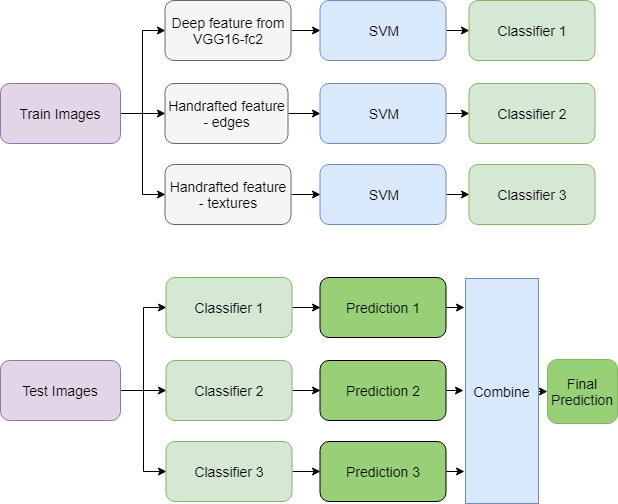
\includegraphics[width=1.0\textwidth]{method_1.png}
	\caption{Mô hình 1: kết hợp probability predictions}
    \label{fig:method_1}
\end{figure}

\section{Mô hình 2: kết hợp features (pre-fusion)}
Với mô hình này, đầu vào cũng có ba nhánh tương tự mô hình thứ nhất, tuy nhiến chúng sẽ không đi song song, thay vào đó các feature rút trích từ ba nhánh sẽ được kết hợp thành một và chỉ huấn luyện một bộ phân lớp duy nhất trên feature đã được kết hợp này.

Trong quá trình test, các feature từ 3 nhánh cũng được kết hợp tương tự và sau đó đi qua bộ phân lớp đã huấn luyện để có kết quả cuối cùng (Hình \ref{fig:method_2}).

\begin{figure}[h!]
	\centering
	\captionsetup{width=0.7\textwidth}
	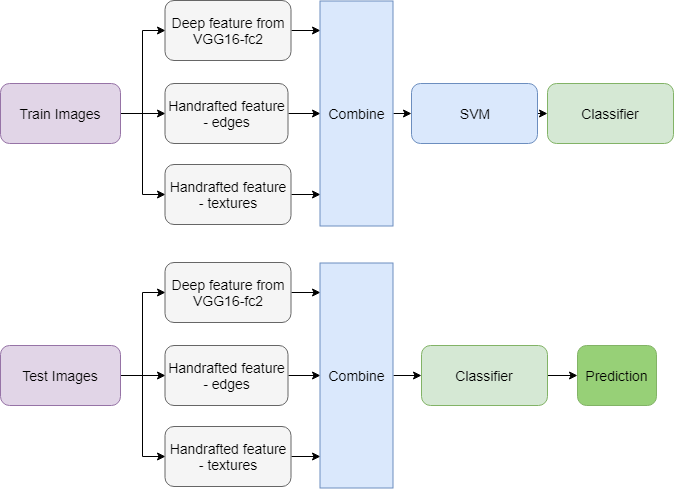
\includegraphics[width=1.0\textwidth]{method_2.png}
	\caption{Mô hình 2: kết hợp features (pre-fusion)}
    \label{fig:method_2}
\end{figure}

\section{Mô hình 3: kết hợp mô hình 1 và 2}
Mô hình này là sự kết hợp của pre-fusion và post fusion bên trên để có thể cho kết quả tốt nhất. Đầu tiên, ảnh huấn luyện sẽ được rút deep feature và các handcrafted features tương tự như trên, sau đó deep feature sẽ dùng để huấn luyện một bộ phân lớp riêng, cùng với đó, deep feature cũng sẽ được kết hợp với các handcrafted features còn lại để huấn luyện một bộ phân lớp riêng (Hình \ref{fig:method_3}).

Với mô hình này, nhánh trên (chỉ dùng deep feature) có thể coi là transfer learning từ một mạng CNN đã được huấn luyện sẵn trên ImageNet và tương ứng với cách dùng bài toán phân lớp đối tượng để giải bài toán phân lớp vật liệu, cùng với đó nhánh 2 kết hợp với các handcrafted features thích hợp sẽ giải quyết được các trường hợp nhập nhằng khi hai đối tượng có cùng hình dạng hay texture (Hình \ref{fig:shape}, \ref{fig:texture}), chính vì thế kết quả phân lớp sẽ tốt hơn.

\begin{figure}[h!]
	\centering
	\captionsetup{width=0.7\textwidth}
	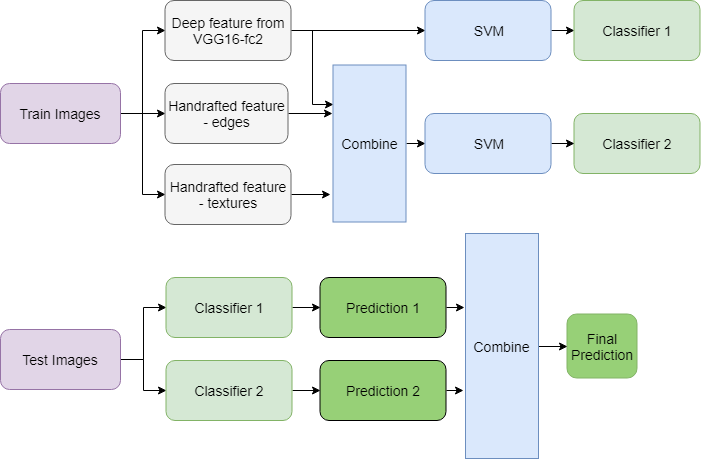
\includegraphics[width=1.0\textwidth]{method_3.png}
	\caption{Mô hình 3: kết hợp mô hình 1 và 2 (full-fusion)}
    \label{fig:method_3}
\end{figure}

\section{Thiết kế một mạng CNN duy nhất tích hợp các mô hình trên vào một}
Cách rút trích features và huấn luyện bằng SVMs như các mô hình trên 
cần lưu trữ một lượng lớn dữ liệu (các feature đã được rút trích). Bên cạnh đó quá trình huấn luyện (bằng SVMs) mất rất nhiều thời gian, tuy nhiên để có một kết quả tốt nhóm cần phải thử nghiệm với rất nhiều bộ tham số khác nhau (của SVMs) nên thời gian và khối lượng tính toán không hề nhỏ, thêm vào đó các bộ phân lớp sau khi đã huấn luyện không thể dùng lại trong lần huấn luyện sau. Thế nên, nhóm đã đề xuất phương pháp kết hợp các mô hình trên vào một mạng CNN duy nhất. Mục tiêu được đề ra là với mạng CNN nhóm sẽ có thể:
\begin{enumerate}
	\item Gộp cả 3 quá trình rút trích feature, huấn luyện và test vào một quá trình duy nhất là huấn luyện mạng CNN này.
	\item Giảm chi phí (không gian lưu trữ, khối lượng và thời gian tính toán)
	\item Khả năng mở rộng và sử dụng lại: mạng CNN có khả năng tự thay đổi tham số để thích ứng tốt hơn với dữ liệu mới (các bộ phân lớp của SVMs thì không thể).
    
Ý tưởng chung của mạng được trình bày trong Hình \ref{}
\end{enumerate}
\chapter{Thực nghiệm và kết quả}
\ifpdf
    \graphicspath{{Chapter5/Chapter5Figs/PNG/}{Chapter5/Chapter5Figs/PDF/}{Chapter5/Chapter5Figs/}}
\else
    \graphicspath{{Chapter5/Chapter5Figs/EPS/}{Chapter5/Chapter5Figs/}}
\fi

Nhóm thực hiện thực nghiệm trên hai tập dữ liệu Ground Terrain in Outdoor Scenes (GTOS) \cite{xue2017differential} và Flicker Material Dataset (FMD) \cite{degol2016geometry}, sau đó so sánh kết quả với các phương pháp state-of-the-art để xem xét sự ảnh hưởng của các handcrafted features trên những dataset khác nhau.
Trên mỗi tập dữ liệu, nhóm đầu tiên thực nghiệm với từng cấu trúc mạng nhóm đề xuất trong phần trên và đánh giá sự hiểu quả của chúng, sau đó so sánh kết quả khi sử dụng các handcrafted feature khác nhau để chỉ ra rằng việc kết hợp handcrafted features càng thích hợp với tập dữ liệu, kết quả sẽ càng tốt. Sau cùng, để có thể thiết kế một CNN có thể tích hợp các phần trên lại với nhau, nhóm thực hiện một số thực nghiệm nhằm hiểu rõ hơn cấu trúc, cách hoạt động của từng layer của một mạng CNN phổ biến và hiểu quả - VGG16 \ref{vgg16}, từ đó có thể dựa trên cấu trúc của mạng này cũng như chọn được những layer thích hợp nhất để xây dựng một CNN riêng.

\section{Môi trường và công cụ thử nghiệm}
Các thực nghiệm trong luận văn này được thực hiện trên PC có cấu hình:
\begin{enumerate}
\item Processor: Intel(R) Core(TM) i7 - 62000U CPU @ 2.40GHz 3.2GHz
\item RAM: 16GB
\item: Opera system: Windows 10 (x64)
\end{enumerate}
Các công cụ được sử dụng bao gồm:
\begin{enumerate}
\item Python 3.6+: Ngôn ngữ lập trình chính để hiện thực các bước thực nghiệm
\item Matlab: Hổ trợ rút trích thông tin về texture và các thực nghiệm nhỏ liên quan
\item scikit-learn: Hổ trợ quá trình huấn luyện các bộ phân lớp với SVM, visualize kết quả 
\item Keras: Hổ trợ việc rút trích deep feature từ CNN và thực hiện các thực nghiệm trên VGG16
\item Tensorflow: back-end cho Keras.
\item OpenCV: Dùng cho việc rút trích các handcrafted features và visualize kết quả
\item Một số công cụ hổ trợ khác
\end{enumerate}

\section{Dataset}
Như đã đề cập bên trên, nhóm sử dụng hai tập dữ liệu để thực nghiệm: GTOS và FMD. 
\paragraph*{}
GTOS là tập dữ liệu mới nhất cho bài toán phân lớp vật liệu, được hoàn thành vào năm 2017 bởi Rutgers ECE Vision Lab. Bao gồm hơn 34000 ảnh thuộc 40 lớp khác nhau được thu thập dưới nhiều điều kiện thời tiết, chiếu sáng khác nhau, đây là một trong những tập dữ liệu đa dạng nhất cho bài toán phân lớp vật liệu.
\paragraph*{}
Ở chiều hướng ngược lại, FMD là một trong những tập dữ liệu phổ biến nhất cho phân loại vật liệu ngay từ những ngày đầu ra đời của bài toán này khoảng đầu năm 2009. Tất cả các ảnh dùng trong hai tập dữ liệu này đều có kích thước 244 x 244.

\begin{figure}[h!]
	\centering
	\captionsetup{width=0.7\textwidth}
    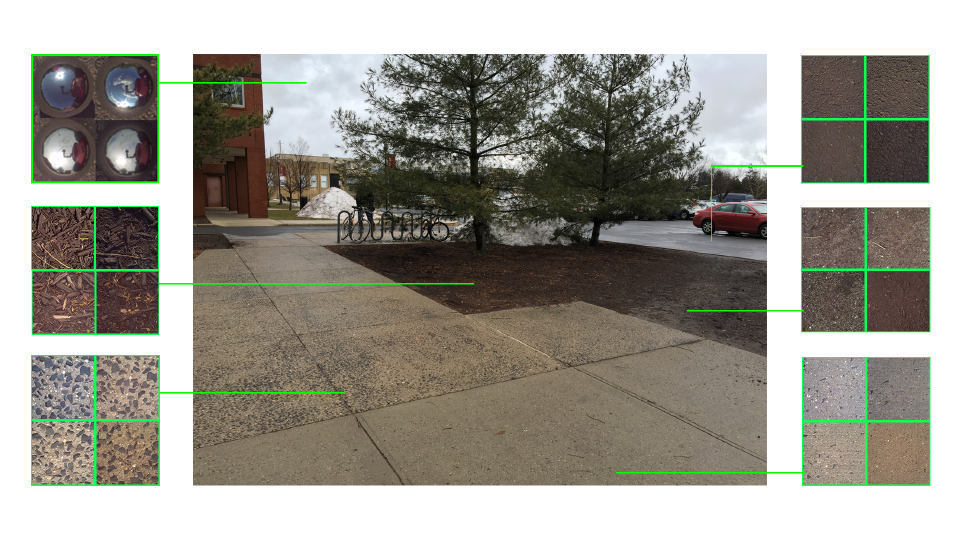
\includegraphics[width=1.0\linewidth]{gtos_dataset.png}
	\caption{Một cảnh ngoài trời được dùng dể lấy các mẫu cho tập dữ liệu GTOS với nhiều góc nhìn nhìn, điều kiện chiếu sáng khác nhau \cite{xue2017differential}}
	\label{fig:gtos_dataset}
\end{figure}

\begin{figure}[h!]
\centering
\captionsetup{width=0.7\textwidth}
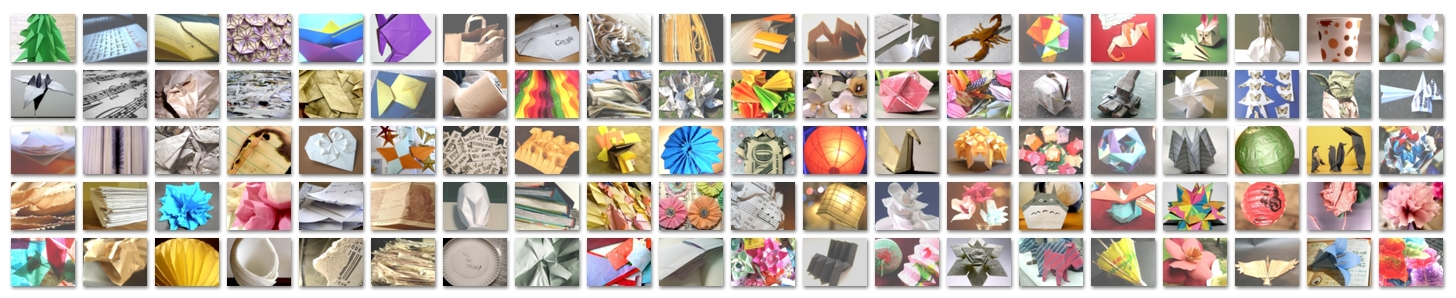
\includegraphics[width=1.0\linewidth]{fmd.png}
\caption{Một tập ảnh từ FMD, đảm bảo sự đa dạng về điều kiện chiếu sáng, bố cục, màu sắc, kết cấu}
\label{fig:fmd}
\end{figure}

\section{Evaluation measures}
Trong cả hai tập dữ liệu, độ chính xác trung bình (mean accuracy) được dùng để đánh giá kết quả cho tất cả các thực nghiệm.

\section{Quá trình thực nghiệm và kết quả}
Nhóm cài đặt các thực nghiệm bằng ngôn ngữ Python với sự hổ trợ của framework scikit-learn và keras (trên nền tensorflow). Mạng VGG16 được huấn luyện sẵn trên ImageNet cũng được dùng cho việc transfer learning và các thực nghiệm khác nhằm hiểu rõ hơn về cách hoạt động của các layer trong CNN.

Tập dữ liệu được chia thành hai tập training và test theo tỷ lệ như các nghiên cứu trước sử dụng: 70\% cho training và 30\% cho test trên tập GTOS, 80\% cho training và 20\% cho test trên tập FMD.

\subsection*{Thực nghiệm với ba mô hình đề xuất}
Đầu tiên nhóm thực hiện rút các handcrafted feature từ ảnh gốc sử dụng các filter thích hợp, bên cạnh đó deep feature cũng được rút từ layer "fc2" của mạng VGG16, sau đó thực hiện huấn luyện các bộ phân lớp ứng với các features khác nhau sử dụng SVMs với nhiều bộ tham số khác nhau, sau cùng dùng các bộ phân lớp này để phân lớp ảnh trên tập test. Probability prediction (trong mô hình 1 và 3) được kết hợp với nhau bằng phép toán trung bình cộng. Và các features được kết hợp với nhau (trong mô hình 2 và 3) bằng phép nối vector (vector concatenation). Các bộ tham số ban đầu (của SVMs) dùng để huấn luyện các bộ phân lớp được ghi nhận lại, từ đó nhóm đánh giá kết quả, điều chỉnh các tham số này thích hợp theo thời gian để có kết quả tốt nhất.

\begin{table}[h!]
  \label{tab:gtos_evaluation}
  \begin{center}
    \resizebox{\linewidth}{!}{
    \begin{tabular}{lccc}
      \toprule[1.0pt]
      \head{Method} 	
      & \head{Deep feature} 
      & \head{Deep+edges} 
      & \head{Deep+edges+textures} \\
      \midrule
      Combine prediction & $75 \pm 1.8$ 	& $75.5 \pm 3.0$  	& $76.3 \pm 1.9$ \\
      Combine features   & $75 \pm 1.8$	& $77.8 \pm 2.5$	& $79.5 \pm 2.5$ \\
      Kết hợp cả hai	   & $75 \pm 1.8$	& $78.9 \pm 2.2$  	& $\textbf{82.2} \pm \textbf{2.3}$\\
      \bottomrule[1.0pt]
    \end{tabular}}
    \captionsetup{width=0.9\textwidth}
    \caption{Kết quả thực nghiệm với các mô hình trên tập GTOS}
  \end{center}
\end{table}

\begin{table}[h!]
  \label{tab:fmd_evaluation}
  \begin{center}
  \resizebox{\linewidth}{!}{
  \begin{tabular}{lccc}
    \toprule[1.0pt]
    \head{Method} 	& \head{Deep feature} 
                    & \head{Deep+edges} 
                    & \head{Deep+edges+textures} \\
    \midrule
    Combine prediction & $74.2 \pm 1.4$ & $75.1 \pm 2.2$  	& $75.5 \pm 2.3$ \\
    Combine features   & $74.2 \pm 1.4$	& $75.3 \pm 1.5$	& $76.3 \pm 1.7$ \\
    Mixed two above    & $74.2 \pm 1.4$	& $75.5 \pm 1.2$  	& $\textbf{77.2} \pm \textbf{0.9}$ \\
    \bottomrule[1.0pt]
  \end{tabular}}
  \captionsetup{width=0.9\textwidth}
  \caption{Kết quả thực nghiệm với các mô hình trên tập FMD}
  \end{center}
\end{table}

Bảng \ref{tab:gtos_evaluation} thể hiện kết quả trên tập GTOS và FMD với ba mô hình đề xuất. Kết quả cho thấy mô hình thứ 3 hoạt động tốt nhất. Hai handcrafted features được dùng thể hiện thông tin về hình dạng và texture hoạt động hiệu quả trên hai tập dữ liệu này. Tuy nhiên, có thể thấy ảnh hưởng của hai features này trên hai tập dữ liệu là khác nhau, trên GTOS hiệu quả của chúng lớn hơn so với trên FMD (đối với cả ba mô hình). Lý do cho điều này được cho là do nhiều ảnh trong FMD là một đối tượng chính nằm trên một background còn GTOS ngược lại, toàn bộ hình đều đồng nhất là một bề mặt duy nhất (Hình \ref{fig:fmd_vs_gtos}). Chính background này khiến thông tin về hình dạng và texture bị ảnh hưởng khác nhiều.

\begin{figure}[h!]
\centering
\captionsetup{width=0.9\textwidth}
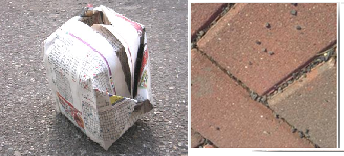
\includegraphics[width=0.75\linewidth]{fmd_vsgtos.png}
\caption{Ảnh từ FMD (bên trái) trong lớp vật liệu "giấy" lại có background là một mặt đường khiến thông tin về texture không còn sự hiệu quả, trong khi ảnh từ GTOS là một bề mặt đồng nhất duy nhất (lớp "Gạch")}
\label{fig:fmd_vs_gtos}
\end{figure}

\begin{table}
\label{tab:comparasion}
\begin{center}
\resizebox{0.6\linewidth}{!}{
\begin{tabular}{lccc}
\toprule[1.0pt]
\head{Method}
				& \head{GTOS} 
                & \head{FMD} \\
\midrule
DAIN & $81.2 \pm 1.7$ & \\
Reflectance  & & $65.5$ \\
SIFT IFV+fc7 & & $69.6 \pm 0.3$ \\
Ours    & $\textbf{82.2}$ & $\textbf{77.2}$ \\
\bottomrule[1.0pt]
\end{tabular}}
\captionsetup{width=0.45\textwidth}
\caption{So sánh kết quả với các phương pháp khác trên 
GTOS và FMD \cite{xue2017differential} \cite{zhang2015reflectance}} \cite{bell2015material}
\end{center}
\end{table}

\begin{figure}[h!]
\centering
\captionsetup{width=0.45\textwidth}
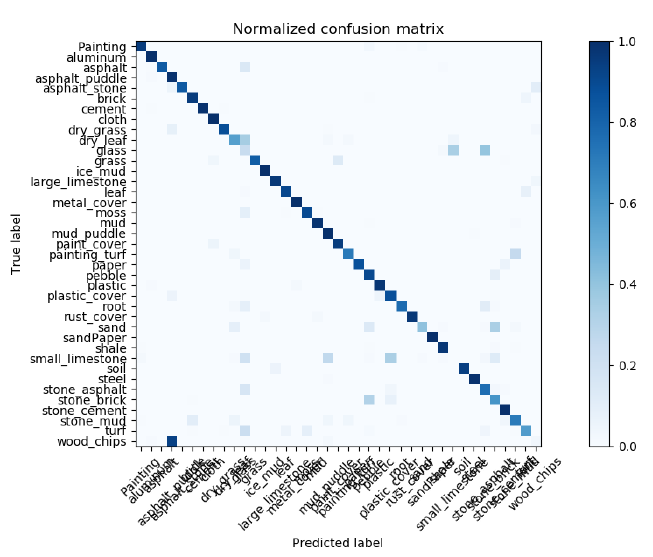
\includegraphics[width=0.9\linewidth]{gtos_confusion.png}
\caption{Normalized confusion matrix trên GTOS}
\label{fig:gtos_confusion}
\end{figure}

\begin{figure}[h!]
\centering
\captionsetup{width=0.45\textwidth}
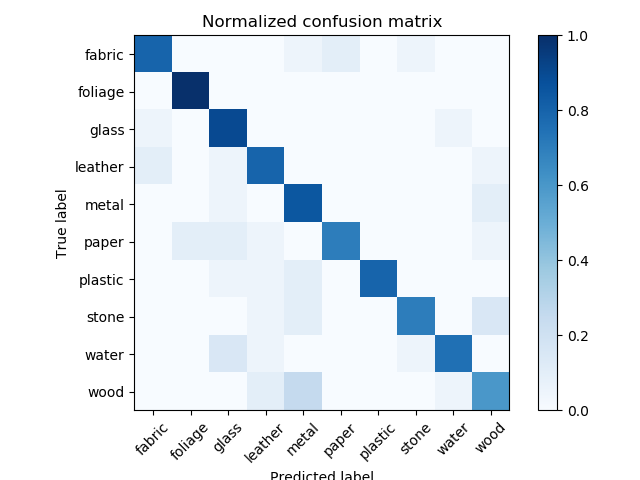
\includegraphics[width=0.9\linewidth]{fmd_confusion.png}
\caption{Normalized confusion matrix trên FMD}
\label{fig:gtos_confusion}
\end{figure}

\begin{table}[h!]
  \label{tab:comparasion}
  \begin{center}
    \resizebox{1.0\linewidth}{!}{
    \begin{tabular}{lr|lr|lr|lr}
      \toprule[1.0pt]
      \head{Classes}
      & \head{Acc.}
      & \head{Classes}
      & \head{Acc.}
      & \head{Classes}
      & \head{Acc.}
      & \head{Classes}
      & \head{Acc.} \\
      \midrule
      painting 		& 0.95 & glass 				& 0.83 & painting turf 	& 0.96 & small limestone 	& 0.87	\\
      aluminum 		& 0.82 & grass 				& 0.98 & paper 			& 0.90 & soil 				& 0.77	\\
      asphalt 		& 0.90 & ice mud 			& 0.84 & pebble			& 0.91 & steel				& 0.96	\\
      asphalt puddle 	& 0.76 & large limestone 	& 0.95 & plastic		& 0.89 & stone asphalt		& 0.40	\\
      asphalt stone 	& 0.60 & leaf 				& 0.99 & plastic cover	& 0.98 & stone brick		& 0.92	\\
      brick 			& 0.99 & metal cover 		& 0.92 & root			& 0.99 & stone cement		& 0.97	\\
      cement 			& 0.71 & moss 				& 0.88 & rust cover		& 0.94 & stone mud			& 0.97	\\
      cloth 			& 0.57 & mud 				& 0.56 & sand			& 0.71 & turf				& 0.94	\\
      dry grass 		& 0.93 & mud puddle			& 0.23 & sand paper		& 0.87 & wood chips			& 0.98	\\
      dry leaf 		& 0.95 & paint cover 		& 0.85 & shale			& 0.97 & 					&		\\
      \bottomrule[1.0pt]
    \end{tabular}}
    \captionsetup{width=0.9\textwidth}
    \caption{Kết quả cho từng lớp vật liệu trên tập GTOS}
  \end{center}
\end{table}

\subsection*{Thực nghiệm với VGG16 (nền tảng để xây dựng một CNN mới)}

\begin{figure}[h!]
\centering
\captionsetup{width=0.9\textwidth}
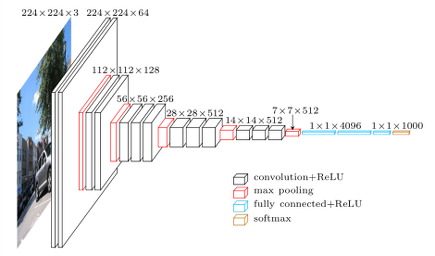
\includegraphics[width=1.0\linewidth]{vgg16.png}
\caption{Cấu trục mạng VGG16 được nhóm dùng để rút trích đặc trưng ở layer 'fc2' và thực hiện các thực nghiệm ở phần thực nghiệm với VGG16}
\label{fig:vgg16}
\end{figure}

Quá trình thực nghiệm với VGG16 qua các bước sau đây:
\begin{enumerate}
\item Fine-tune VGG16: Thay fully-connected layer cuối cùng để đầu ra là 39 lớp (trên GTOS) thay vì 1000 lớp (trên ImageNet) và huấn luyện lại giá trị tham số của layer này, sau đó huấn luyện lại tất cả các layer để so sánh kết quả.
\item Tìm hiểu sự ảnh hưởng của các layer trong mạng bằng cách bỏ bớt layer trong mạng, quan sát ảnh hưởng của các layer này trên kết quả thu được.
\item QUa quan sát từ bước 2 và dựa trên nền của VGG16 chọn các layer thích hợp để xây dựng một mạng CNN ít layer hơn nhưng đạt kết quả xấp xĩ.
\end{enumerate}

Hiện tại, khi đang viết luận văn này, nhóm vẫn đang thực nghiệm ở bước một, kết quả sau khi fine-tune trên GTOS cho thấy thời gian giảm 1/3 so với sử dụng SVM (bao gồm thời gian rút trích đặc trưng, huấn luyện và test), không cần tốn không gian lưu trữ đặc trưng và độ chính xác giảm từ $82.2\%$ xuống còn $79.8\%$.

\def\baselinestretch{1}
\chapter{Kết luận và hướng phát triển}
\ifpdf
    \graphicspath{{Conclusions/ConclusionsFigs/PNG/}{Conclusions/ConclusionsFigs/PDF/}{Conclusions/ConclusionsFigs/}}
\else
    \graphicspath{{Conclusions/ConclusionsFigs/EPS/}{Conclusions/ConclusionsFigs/}}
\fi

\def\baselinestretch{1.66}
\section{Kết quả đạt được}
Sau giai đoạn luận văn, nhóm đã áp dụng được các kiến thức chuyên ngành đã được học vào bài toán phân lớp vật liệu. Sau quá trình tìm hiểu, tổng hợp các nghiên cứu trước, nhóm đã nắm được các phương pháp cơ bản hiện có cho bài toán, dựa vào đó đưa ra một số mô hình nhằm cải thiện kết quả. Báo cáo đã trình bày những mô hình nhóm đề xuất cũng như quá trình cài đặt, thử nghiệm đánh giá các mô hình này trên những tập dữ liệu khác nhau.

\section{Hướng phát triển}
Với kết quả hiện tại của đề tài, nhóm nhận thấy các mô hình đề xuất còn có nhiều hướng phát triển, chỉnh sửa nhằm cải thiện cả về độ chính xác, hiệu suất, tài nguyên sử dụng. Bên dưới là một số hướng phát triển tiếp theo cho đề tài mà nhóm dự định thực hiện.
\begin{enumerate}
\item Tiếp tục các thực nghiệm với mạng VGG16 để có một cái nhìn sâu hơn về cách các layer của nó hoạt động, từ đó có thể thiết kế một mạng mới thích hợp cho bài toán hiện tại. Điều này giúp tích kiệm chi phí huấn luyện các mô hình trên đồng thời cũng tăng độ thích ứng của mô hình với dữ liệu mới (so với việc dùng SVMs để huấn luyện các bộ phân lớp)
\item Thay đổi cách kết hợp features và probability prediction như đã trình bày trong ba mô hình trên. Có thể kết hợp theo trọng số thay vì dùng phép nối vector và trung bình cộng như hiện tại.
\item Kết hợp thêm các thông tin khác có thể lấy từ ảnh (ví dụ như thông tin về góc nhìn - một mẫu với nhiều góc nhìn khác nhau, nghiên cứu \cite{xue2017differential} đã cho thấy thông tin này rất giá trị trong bài toán phân lớp vật liệu)
\end{enumerate}
%%% ----------------------------------------------------------------------

% ------------------------------------------------------------------------

%%% Local Variables: 
%%% mode: latex
%%% TeX-master: "../thesis"
%%% End: 


\backmatter  
%\appendix
%\include{Appendix1/appendix1}
%\include{Appendix2/appendix2}

\bibliographystyle{IEEEtran}
\bibliography{References/references}

%\bibliographystyle{Classes/jmb} % bibliography style
%\renewcommand{\bibname}{References} % changes default name Bibliography to References
%\bibliography{security} % References file

\end{document}
